\documentclass[12pt,letterpaper]{article}

% ── Layout ────────────────────────────────────────────────────────────────────
\usepackage[margin=1in]{geometry}
\usepackage{setspace}
\setstretch{1.5}
\usepackage{microtype}
\usepackage{comment}

% ── Math & Physics ────────────────────────────────────────────────────────────
\usepackage{amsmath, amssymb, mathtools}
\usepackage{siunitx}

% ── Figures & Tables ──────────────────────────────────────────────────────────
\usepackage{graphicx}
\usepackage{float}
\usepackage{caption}
\usepackage{subcaption}
\usepackage{booktabs}

% ── References & Links ────────────────────────────────────────────────────────
\usepackage[numbers,sort&compress]{natbib}
\bibliographystyle{unsrt}
\usepackage[colorlinks=true, linkcolor=blue!60!black,
            citecolor=blue!60!black, urlcolor=blue!60!black]{hyperref}

% ── Misc ──────────────────────────────────────────────────────────────────────
\usepackage{xcolor}
\usepackage{enumitem}
\usepackage{lineno}
\usepackage{verbatim}
\linenumbers

% ── Custom commands ───────────────────────────────────────────────────────────
\newcommand{\gcm}{\,\mathrm{g\,cm^{-2}}}
\newcommand{\mGyday}{\,\mathrm{mGy\,day^{-1}}}
\newcommand{\mSvday}{\,\mathrm{mSv\,day^{-1}}}
\newcommand{\keVum}{\,\mathrm{keV\,\mu m^{-1}}}
\newcommand{\Qeff}{Q_\mathrm{eff}}
\newcommand{\LETd}{\overline{L}_D}
\newcommand{\REID}{\mathrm{REID}}
\newcommand{\code}[1]{\texttt{#1}}

% ─────────────────────────────────────────────────────────────────────────────
\title{An open-source GCR dosimetry pipeline for Mars mission risk assessment:\\
       organ-specific REID, SEP acute hazard, and dual-use\\
       proton therapy RBE benchmarking}

\author{Aryan Hemendra Shah\\[4pt]
  \small University of Miami\\
  \small \href{mailto:ahs222@miami.edu}{ahs222@miami.edu}\\
  \small ORCID: \href{https://orcid.org/0009-0008-0518-428X}{0009-0008-0518-428X}
}
\date{\today}
% ─────────────────────────────────────────────────────────────────────────────

\begin{document}
\maketitle

% ── Abstract ─────────────────────────────────────────────────────────────────
\begin{abstract}

We describe \textsc{gcr-dosimetry-pipeline}, an open-source Python package for
estimating galactic cosmic ray (GCR) radiation exposure and cancer risk on
crewed deep-space trajectories.
The pipeline uses Gleeson--Axford force-field solar modulation \citep{gleeson1968}
with per-species local interstellar spectra \citep{vos2015, boschini2020}.
GCR flux is transported through slab shielding via continuous-slowing-down
approximation (CSDA) with effective-charge stopping power scaling; secondary
neutron dose equivalent comes from a pre-computed HZETRN table \citep{slaba2014}.
Organ-specific cancer risk is estimated as radiation exposure in incidence of
death (REID) across eleven organs at ICRP-89 tissue depths \citep{cucinotta2013}.

The pipeline's per-species normalization factors are calibrated to the
MSL/RAD cruise-phase measurement of $1.84 \pm 0.33$~mGy/day
\citep{zeitlin2013} at $16\gcm$ aluminum, and the shielding-depth
dependence and material ratio are independently compared against HZETRN
benchmark data \citep{slaba2014, mrigakshi2013}, showing agreement within
the stated benchmark uncertainties ($\lesssim 20\%$ on absolute dose).
A Solar Energetic Particle module estimates BFO absorbed dose from three
canonical events using Band-function spectra \citep{tylka2006};
the August~1972 event requires $>30\gcm$ aluminum to fall below the
NASA 30-day limit of $250$~mGy.

Global physics and radiobiological uncertainties are propagated via Latin
Hypercube Sampling over eight parameters, yielding a median REID of $5.0\%$ with p5--p95 bounds of $1.3\%$--$16.9\%$
(13.4$\times$ spread, typical for this class of analysis) for a 35-year-old
male crew member on a 259-day Earth--Mars transit at $16\gcm$ aluminum.
Variance decomposition shows that the quality factor scale parameter
($76\%$ of REID variance) and DDREF ($7\%$) together dominate output
uncertainty, while all GCR physics parameters together contribute $<9\%$,
confirming that better transport physics alone will not narrow REID bounds
without matching progress in high-LET human radiobiology.

Per-species $\LETd$ decomposition reveals that carbon ions contribute
approximately $59\%$ of unshielded GCR absorbed dose at a field
$\LETd \approx 18.7\keVum$, yielding $\Qeff = 2.60$, consistent with
the MSL/RAD measured value of $2.62 \pm 0.14$ within measurement
uncertainty.
Sixteen g/cm$^2$ of aluminum reduces the carbon fraction to $31\%$
and the field $\LETd$ to $4.1\keVum$, bridging toward the LET range of
clinical proton therapy Bragg peaks.
Wedenberg \citep{wedenberg2013} and McNamara \citep{mcnamara2015} proton RBE
models agree with OpenTOPAS-RBE scorer output to within mean absolute error
$<10^{-3}$ for V79 cells (self-consistency check for clinical cell lines),
enabling consistent comparison of space and clinical radiation quality factors
from a single codebase.
All source code, 103 automated tests, validation data, and TOPAS geometry
files are freely available at \url{https://github.com/aryanhshah8/gcr-dosimetry-pipeline}.

\end{abstract}

\textbf{Keywords:}
galactic cosmic rays; Mars mission dosimetry; radiation risk; REID;
solar energetic particles; proton therapy RBE; uncertainty quantification;
open-source

% ─────────────────────────────────────────────────────────────────────────────
\section{Introduction}
\label{sec:intro}

Deep-space human exploration beyond low-Earth orbit exposes crew members to
galactic cosmic rays (GCR) and solar energetic particles (SEP) at fluence
rates and energies far exceeding the shielding capacity of current crew
vehicles.
The GCR environment at 1--1.5~AU consists of protons, helium, and heavier ions
(the so-called HZE particles) spanning kinetic energies from a few
hundred MeV/n to tens of GeV/n, with the peak in biological effectiveness
occurring near the energy range where stopping power is highest.
A round-trip crewed Mars mission (transit + surface stay) of approximately
900 days is estimated to deliver a total effective dose of the order
$1$--$2$~Sv \citep{zeitlin2013}, which, depending on crew demographics and
the risk model used, implies a radiation-induced cancer mortality probability
that may approach or exceed NASA's current career limit \citep{cucinotta2013}.

Quantifying this risk accurately requires several components that are not
trivially combined: a calibrated GCR spectral model responsive to solar
modulation, organ-resolved dose transport through shielding and tissue,
a cancer risk model that accounts for the high-LET quality of HZE radiation,
and a quantitative uncertainty analysis that separates reducible physics
uncertainties from the fundamentally larger radiobiological unknowns.
Existing tools (HZETRN \citep{wilson1991}, OLTARIS, and Geant4/TOPAS) address
subsets of these requirements with greater physical rigor than the present
work, particularly in the treatment of nuclear fragmentation.
However, they are not all openly available, not installable via pip, and do not
in general integrate physics transport, organ REID, SEP risk, and uncertainty
quantification into a single executable workflow.

Separately, a parallel development in radiation oncology has produced
validated LET-dependent RBE models for clinical proton therapy
\citep{wedenberg2013, mcnamara2015}.
Proton therapy currently uses a fixed biological effectiveness factor of RBE
$= 1.1$ relative to photons, despite growing evidence that the RBE in the
distal Bragg peak, where LET is highest, may significantly exceed this value,
particularly for CNS and late-responding tissues with low
$\alpha/\beta$ \citep{paganetti2014}.
The physical quantity linking space radiation and proton therapy is the
dose-averaged LET ($\LETd$): the same quantity that determines the GCR
effective quality factor $\Qeff$ via ICRP-60 also drives deviations of proton
therapy RBE from 1.1 via the Wedenberg and McNamara models.
Yet, to our knowledge, no open tool has quantitatively demonstrated this
connection across both domains.

Here we present \code{gcr-dosimetry-pipeline}, a Python package that, within
the limitations stated in Section~\ref{sec:discuss_limits}:
\begin{enumerate}[leftmargin=*, label=\arabic*.]
  \item Generates six-species GCR spectra with force-field solar modulation
        calibrated to MSL/RAD cruise-phase measurements;
  \item Transports spectra through slab shielding via CSDA + nuclear
        attenuation, with secondary neutrons from a validated table;
  \item Computes organ-specific absorbed dose and dose equivalent for
        eleven organs at ICRP-89 tissue depths;
  \item Estimates REID via the Cucinotta (2013) organ EAR/ERR model with
        CDC 2020 US life tables;
  \item Quantifies SEP acute BFO absorbed dose from Band-function spectra
        for three canonical events;
  \item Propagates global uncertainty via 8-parameter Latin Hypercube
        Sampling and decomposes output variance by parameter;
  \item Benchmarks Wedenberg and McNamara RBE models against OpenTOPAS-RBE
        reference data for three clinical cell lines.
\end{enumerate}

The pipeline is not intended as a replacement for HZETRN or Geant4 in
high-fidelity mission analysis.
Its value is transparency, reproducibility, and integrated uncertainty
quantification — properties that closed or proprietary codes generally
do not offer.
Mission planners who need to quickly prototype shielding scenarios can
run the full GCR, SEP, and REID workflow from a single install without
requiring HZETRN access or a Geant4 build.
Researchers studying where uncertainty reduction effort should be
directed will find the LHS variance decomposition directly useful: the
finding that physics parameters together contribute less than 9\% of
REID variance while radiobiological parameters contribute more than 70\%
is difficult to extract from existing closed tools.
Students and researchers entering either the space radiation or proton
therapy field also gain a readable, fully tested reference implementation
rather than a black-box executable.
The methods, results, discussion of limitations, and reproducibility
instructions are described in the sections that follow.


% ─────────────────────────────────────────────────────────────────────────────
% Methods — include detailed section from separate file
% ─────────────────────────────────────────────────────────────────────────────
% DETAILED METHODS SECTION
% gcr-dosimetry-pipeline — Life Sciences in Space Research submission
% ─────────────────────────────────────────────────────────────────────────────

\section{Methods}
\label{sec:methods}

All computation is implemented in Python~3.9+ as the open-source package
\code{gcr-dosimetry\discretionary{-}{}{-}pipeline}.
The pipeline is structured as a sequence of composable modules, each responsible
for one physical layer of the problem:
spectrum generation~(\S\ref{sec:spectrum}),
slab transport~(\S\ref{sec:transport}),
organ dose~(\S\ref{sec:organdose}),
cancer risk~(\S\ref{sec:reid}),
SEP acute hazard~(\S\ref{sec:sep}),
uncertainty propagation~(\S\ref{sec:uq}),
and RBE benchmarking~(\S\ref{sec:rbemethods}).
Where simplifying assumptions are made (particularly in the transport
layer), we state them explicitly and discuss their domain of validity.

% ─────────────────────────────────────────────────────────────────────────────
\subsection{Mission Trajectory Model}
\label{sec:trajectory}

A Hohmann-transfer trajectory from Earth (1.0~AU) to Mars (1.524~AU) is
generated by computing heliocentric distance as a function of mission elapsed
time, $r(t)$, using Keplerian orbital mechanics:
\begin{equation}
  r(t) = \frac{a(1-e^2)}{1 + e\cos\theta(t)},
  \label{eq:orbit}
\end{equation}
where $a = (r_\oplus + r_\mathrm{Mars})/2 = 1.262$~AU is the semi-major axis
and $e = (r_\mathrm{Mars} - r_\oplus)/(r_\mathrm{Mars} + r_\oplus) = 0.208$
is the eccentricity of the transfer ellipse.
Transit duration is fixed at 259~days (one half-period of the transfer orbit).
The heliocentric distance enters the dose rate only through the solar modulation
potential $\phi(t)$; direct geometric flux dilution as $r^{-2}$ is not applied
separately because the force-field modulation already encodes the energy
dependence of solar wind effects at the relevant energies.

For surface exposure at Mars, a constant heliocentric distance of 1.524~AU is
assumed with an Olympus Mons atmospheric overburden of approximately
$22\,\mathrm{g\,cm^{-2}}$, though the present paper focuses on the transit
phase where the SEP and shielding comparisons are most directly constrained
by MSL/RAD data.

% ─────────────────────────────────────────────────────────────────────────────
\subsection{Solar Modulation Potential}
\label{sec:phi}

The time-resolved solar modulation potential $\phi(t)$ is obtained from the
Usoskin et~al.\ (2017) database, which provides monthly $\phi$ values
reconstructed from ground-level neutron monitor count rates
back to 1936.
For the MSL transit period (2011~November -- 2012~July), values cluster around
$\phi \approx 481 \pm 50$~MV corresponding to an ascending phase toward
solar maximum.
For future mission scenarios, $\phi$ is frozen at a user-specified
value representing an assumed solar activity level.

We note a known limitation of the Usoskin database: systematic offsets between
different neutron monitor stations can introduce $\pm 50$--$100$~MV uncertainty
in the absolute $\phi$ calibration.
This uncertainty is explicitly propagated in Section~\ref{sec:uq} via a
multiplicative scale parameter on $\phi$.

% ─────────────────────────────────────────────────────────────────────────────
\subsection{GCR Spectrum Generation}
\label{sec:spectrum}

\subsubsection{Force-Field Modulation}
\label{sec:forcefield}

Solar modulation of the GCR flux is computed using the Gleeson--Axford (1968)
force-field approximation, which treats the heliosphere as a spherically
symmetric potential well of depth $\phi$ (in MV) through which particles must
propagate diffusively.
For an ion of charge $Z$ and mass number $A$, the modulated differential flux
at kinetic energy per nucleon $E$ is:
\begin{equation}
  J(E, \phi) = J_\mathrm{LIS}(E + \delta E)
  \cdot \frac{E(E + 2E_0)}{(E + \delta E)(E + \delta E + 2E_0)},
  \label{eq:ff}
\end{equation}
where $E_0 = 938.272$~MeV is the proton rest-mass energy,
$\delta E = (Z/A)\,\phi$ (MeV/nucleon) is the kinetic energy shift due to
solar deceleration, and $J_\mathrm{LIS}$ is the local interstellar spectrum
described in Section~\ref{sec:lis}.
The ratio in Eq.~\eqref{eq:ff} is the Jacobian of the energy transformation,
ensuring flux conservation.

The force-field approximation is known to be accurate for rigidities above
approximately $1$~GV ($E/n \gtrsim 200$~MeV for protons) and for solar
modulation potentials in the range $200$--$1500$~MV \citep{usoskin2017}.
At lower energies, charge-sign dependent drift effects (important for
anomalous cosmic rays and at solar minimum) are not captured.
For this application, where dose is dominated by particles above a few
hundred MeV/n, this limitation is not expected to significantly change
the results.

\subsubsection{Local Interstellar Spectra}
\label{sec:lis}

\paragraph{Protons.}
The LIS for protons follows the parameterization of Vos \& Potgieter \cite{vos2015}:
\begin{equation}
  J_\mathrm{LIS}^\mathrm{H}(E) = C_\mathrm{H}
  \cdot \frac{(E_\mathrm{GeV} + 0.67)^{-3.93}}{\beta^2},
  \label{eq:lis_proton}
\end{equation}
where $C_\mathrm{H} = 1.9 \times 10^4$~cm$^{-2}$~s$^{-1}$~MeV$^{-1}$~sr$^{-1}$,
$E_\mathrm{GeV} = E / 1000$ is the kinetic energy in GeV/nucleon, and
$\beta = v/c$ is the particle velocity normalized to the speed of light.
The $\beta^{-2}$ factor reflects the well-known ``1/v'' rise in flux at
low energies due to the slowing of particles by ionization energy loss.
This parametrization was fit to Voyager~1 and PAMELA measurements and
is considered one of the more reliable proton LIS forms currently available,
though low-energy Voyager constraints remain subject to ongoing refinement
as the spacecraft continues to recede from the heliosphere.

\paragraph{Helium.}
The helium LIS uses the same functional form with species-specific parameters
($C_\mathrm{He} = 1.82 \times 10^3$, spectral index $\alpha_\mathrm{He} = 2.78$,
offset $= 0.62$), which produces a He/H ratio of approximately $0.096$ at
$1$~GeV/n, consistent with ACE CRIS measurements \citep{stone1998}.
The harder helium spectrum ($\alpha_\mathrm{He} = 2.78$ vs.\ proton
$\alpha_\mathrm{H} = 3.93$) means helium contributes proportionally more
flux at high energies.

\paragraph{Heavy ions.}
Carbon, oxygen, silicon, and iron LIS parametrizations follow the per-species
HelMod model of Boschini et al.\ \cite{boschini2020}, which provides explicit spectral indices
and normalizations for each species fit to ACE, PAMELA, and AMS-02 data:
\begin{equation}
  J_\mathrm{LIS}^{(s)}(E_n) = C_s \cdot
  \frac{(E_\mathrm{GeV/n} + \delta_s)^{-\alpha_s}}{\beta^2}.
  \label{eq:lis_heavy}
\end{equation}
Iron is particularly important: with $\alpha_\mathrm{Fe} = 2.65$ (flatter than
protons), there is significantly more high-energy iron flux, and via
$Z^2$ scaling of stopping power, iron contributes disproportionately to
dose equivalent at all depths.
The adopted spectral parameters are summarized in Table~\ref{tab:lis_params}.

\begin{table}[H]
  \centering
  \caption{LIS spectral parameters used in \code{gcr/spectrum.py}.
           Proton and helium from Vos \& Potgieter \cite{vos2015}; heavy ions from
           Boschini et al.\ \cite{boschini2020}.}
  \label{tab:lis_params}
  \begin{tabular}{lcccl}
    \toprule
    Species & $C_s$ & $\alpha_s$ & $\delta_s$ (GeV/n) & Primary source \\
    \midrule
    H       & $1.90\times10^4$ & 3.93 & 0.67 & Vos \& Potgieter (2015) \\
    He      & $1.82\times10^3$ & 2.78 & 0.62 & Vos \& Potgieter (2015) \\
    C       & $2.50\times10^2$ & 2.72 & 0.50 & Boschini et al.\ (2020) \\
    O       & $1.80\times10^2$ & 2.69 & 0.50 & Boschini et al.\ (2020) \\
    Si      & $3.00\times10^1$ & 2.70 & 0.50 & Boschini et al.\ (2020) \\
    Fe      & $4.30\times10^0$ & 2.65 & 0.50 & Boschini et al.\ (2020) \\
    \bottomrule
  \end{tabular}
\end{table}

\paragraph{Per-species normalization.}
\label{sec:calib}
A set of empirical calibration factors $f_s$ are applied to each species
flux after modulation:
\begin{equation}
  J_s(E, \phi) \leftarrow f_s \cdot J_s(E, \phi),
  \label{eq:calib}
\end{equation}
with values $f_\mathrm{H} = 0.590$, $f_\mathrm{He} = 0.082$,
$f_\mathrm{C} = 1.980$, $f_\mathrm{O} = 0.016$,
$f_\mathrm{Si} = 0.025$, $f_\mathrm{Fe} = 0.002$.
These factors were fit by minimizing the squared difference between the
pipeline's predicted dose rate and the MSL/RAD cruise measurement
$\dot{D} = 1.84$~mGy/day at $16\,\mathrm{g\,cm^{-2}}$ aluminum,
with $\phi = 481$~MV.
We emphasize that this constitutes a \emph{calibration step}, not an
independent prediction: the pipeline is calibrated to one operational
flight measurement and then used to extrapolate to other shielding
depths, materials, launch dates, and mission types.
Accordingly, the agreement between the pipeline and MSL/RAD at the
calibration point should not be interpreted as a validation of the
underlying physical model; the independent validation evidence consists
of the shielding-depth dependence, the material ratio, and the temporal
modulation (Section~\ref{sec:validation}).

Several normalization values depart substantially from unity and merit
comment.
$f_\mathrm{He} = 0.082$ and $f_\mathrm{O} = 0.016$ suppress helium and
oxygen to below 10\% of their LIS predictions, while
$f_\mathrm{C} = 1.980$ nearly doubles the carbon flux.
These large corrections arise from a fundamental underdetermination:
six species-level free parameters are fit to a single total dose scalar.
Many combinations of $\{f_s\}$ reproduce $\dot{D} = 1.84$~mGy/day
while distributing dose very differently among species.
The physical plausibility of individual $f_s$ values can be partially
assessed against ACE/CRIS measurements of GCR composition near
1~AU \citep{stone1998}, which report He/H~$\approx 0.096$ at
$\sim\!500$~MeV/n — consistent with the unmodified LIS prediction of
$\approx 0.096$, suggesting $f_\mathrm{He}$ should be near unity rather
than $0.082$.
The factor-of-five discrepancy implies that the optimizer is
suppressing helium not because the helium LIS is wrong, but because
it is trading helium flux against carbon flux (which has a
$\sim\!36\times$ higher stopping power per nucleon and therefore
disproportionate leverage on total dose) to satisfy the single-point
constraint.
$f_\mathrm{C} > 1$ when ACE/CRIS abundance ratios suggest the
Boschini (2020) carbon LIS is already near the measured value is
most plausibly explained by the missing magnesium contribution
(Section~\ref{sec:discuss_limits}): if Mg ($Z=12$, absent from the
model) accounts for $\sim\!3\%$ of dose, the optimizer inflates
whatever high-LET species has the most flexibility — here, carbon.
The normalization factors are therefore best understood as a joint
correction for missing species, absolute LIS normalization offsets, and
CSDA dose-model systematics across the species mix — not as independent
corrections to each species' intrinsic flux.
A species-resolved calibration using the MSL/RAD per-species dose
fractions \citep{zeitlin2013} would directly constrain each $f_s$
and is a planned extension of this work.

A comparison with the NASA Space Radiation Laboratory (NSRL) GCR
simulator reference field \citep{slaba2016} provides independent
context for the per-species dose fractions the pipeline produces.
Table~\ref{tab:species_compare} shows the charge-group dose breakdown
from the pipeline at the calibration geometry against the NSRL
reference at comparable conditions.

\begin{table}[H]
  \centering
  \small
  \caption{Per-charge-group absorbed dose fractions at shielded
           geometries: pipeline output vs.\ the NSRL GCR simulator
           reference field \citep{slaba2016}.
           The two configurations differ by $4\,\mathrm{g\,cm^{-2}}$
           of aluminum and by solar conditions (ascending vs.\ minimum);
           neither difference can account for the
           $\sim\!4\times$ excess in the pipeline HZE fraction.}
  \label{tab:species_compare}
  \begin{tabular}{lccc}
    \toprule
    Particle class
      & \multicolumn{1}{p{3.2cm}}{\centering Pipeline \\ $16\gcm$ Al, $\phi=481$~MV}
      & \multicolumn{1}{p{3.2cm}}{\centering NSRL GCR reference \\ $20\gcm$ Al, solar min \citep{slaba2016}} \\
    \midrule
    $Z=1$ (protons)  & 46.7\% & 73.3\% \\
    $Z=2$ (helium)   & 16.8\% & 19.2\% \\
    $Z>2$ (HZE)      & 30.9\% &  7.6\% \\
    \bottomrule
    \multicolumn{3}{l}{\small NSRL fractions exclude $\pi$/EM cascades
      and heavy-target fragments.} \\
  \end{tabular}
\end{table}

The pipeline's proton fraction is $\sim\!27$ percentage points below
the NSRL reference, while the HZE fraction is approximately four
times higher.
Carbon ions alone account for $31.2\%$ of dose at $16\gcm$ Al in the
pipeline, yet the total HZE fraction in the NSRL reference is $7.6\%$.
This confirms, quantitatively, that the normalization factors are
producing species fractions well outside the physically expected
range — a direct consequence of the underdetermined single-point
calibration described above.
The helium fraction ($16.8\%$ vs $19.2\%$) is the one charge group
where agreement is reasonable, consistent with the unmodified
LIS He/H ratio already being close to the ACE/CRIS measurement
\citep{stone1998}.

% ─────────────────────────────────────────────────────────────────────────────
\subsection{Charged Particle Transport}
\label{sec:transport}

\subsubsection{Stopping Power and CSDA Range}
\label{sec:bethe}

Energy loss of a heavy ion traversing a material slab is computed in the
continuous-slowing-down approximation (CSDA), which treats the particle as
losing energy continuously according to its instantaneous stopping power.
The stopping power for an ion of charge $Z$ and velocity $\beta$ is modeled as:
\begin{equation}
  S(E/A,\, Z) = z_\mathrm{eff}^2(E/A,\, Z) \cdot S_p(E/A),
  \label{eq:stopping}
\end{equation}
where $S_p(E/A)$ is the proton stopping power at the same energy per nucleon,
and $z_\mathrm{eff}$ is the Barkas effective charge, which accounts for
partial charge-state stripping at energies below approximately
$1$~GeV/n \citep{barkas1956}:
\begin{equation}
  z_\mathrm{eff}(E/A,\, Z) = Z \left[1 - \exp\!\left(-125\beta Z^{-2/3}\right)\right].
  \label{eq:zeff}
\end{equation}
At energies above $\sim 1$~GeV/n, $z_\mathrm{eff} \to Z$ and the scaling
reduces to the familiar $Z^2$ form.
Proton stopping powers for aluminum, polyethylene, water, and tissue are
tabulated at 500 logarithmically spaced energy points from 1~MeV to
$10^5$~MeV using NIST PSTAR/ASTAR data, and interpolated via cubic spline.

The CSDA range is:
\begin{equation}
  R(E) = \int_0^E \frac{dE'}{S(E', Z)}\,,
  \label{eq:range}
\end{equation}
evaluated by numerical integration of the stopping power table.
The exit energy of an ion entering a slab of areal density $x\,[\mathrm{g\,cm^{-2}}]$
is obtained by inverting the range relation:
\begin{equation}
  E_\mathrm{out} = R^{-1}\!\bigl(R(E_\mathrm{in}) - x_\mathrm{eff}\bigr),
  \label{eq:eout}
\end{equation}
where $x_\mathrm{eff} = x \cdot Z^2/A$ is the effective proton-equivalent
areal density for heavy ions.
If $R(E_\mathrm{in}) < x_\mathrm{eff}$, the particle is stopped ($E_\mathrm{out} = 0$).

\subsubsection{Nuclear Interaction Attenuation}
\label{sec:nuclear}

In addition to ionization energy loss, heavy ions undergo inelastic nuclear
interactions with the shielding material.
These are modeled via an exponential fluence attenuation:
\begin{equation}
  \Phi_s(E, x) = \Phi_s^{(0)}(E) \cdot \exp\!\left(-\frac{x}{\lambda_s}\right),
  \label{eq:attenuation}
\end{equation}
where $\lambda_s$ is a species-dependent nuclear interaction mean free path.
Values are taken from Wilson et~al.\ (1991) for aluminum; for polyethylene,
$\lambda_s$ is scaled by the material density ratio and effective nuclear charge.
This exponential approximation does not account for the secondary fragment
spectrum produced in nuclear fragmentation reactions.
For iron and silicon, this approximation becomes increasingly crude above
$\sim 30\,\mathrm{g\,cm^{-2}}$, where fragmentation produces significant
lighter-ion secondaries (primarily C and O) that are themselves biologically
relevant.
A more accurate treatment would require a full nuclear reaction network
(as implemented in HZETRN or Geant4/TOPAS), and this represents the
primary physical limitation of the current transport model.

The full transport step for species $s$ through shielding $x$ is:
\begin{align}
  \Phi_s^\mathrm{out}(E) &=
    \mathcal{T}_s\bigl[\Phi_s^\mathrm{in}(E), x\bigr] \notag \\
  &= \Phi_s^\mathrm{in}(E_\mathrm{in}(E, x)) \cdot
     \exp\!\left(-\frac{x}{\lambda_s}\right) \cdot
     \frac{E_\mathrm{in}(E_\mathrm{in} + 2E_0)}{E(E + 2E_0)},
  \label{eq:transport}
\end{align}
where the final ratio is a flux density Jacobian correcting for the change
in energy bin width after deceleration.

\subsubsection{Secondary Neutron Production}
\label{sec:neutrons}

Spallation reactions between GCR ions and shielding nuclei produce secondary
neutrons that contribute meaningfully to dose equivalent, particularly in
aluminum where the cross-sections are relatively high.
Rather than tracking individual neutron histories (which would require a
full Monte Carlo or deterministic neutron transport code), neutron
dose equivalent is estimated from a pre-computed look-up table of the form:
\begin{equation}
  \dot{H}_n(x, \phi, \mathrm{mat}) = \dot{H}_n^\mathrm{Al}(\phi) \cdot
  f_\mathrm{mat} \cdot g(x),
  \label{eq:neutron}
\end{equation}
where $\dot{H}_n^\mathrm{Al}(\phi)$ is the neutron dose equivalent rate for
aluminum at a reference thickness, $f_\mathrm{mat}$ is a material-dependent
yield factor (polyethylene $\approx 0.72\times$ aluminum due to lower spallation
cross-sections), and $g(x)$ is an interpolated depth-dependence from the
HZETRN benchmark dataset of Slaba et al.\ \cite{slaba2014}.
The neutron quality factor is taken as $Q_n = 10$ (ICRP-60), which is a
weighted average over the neutron energy spectrum in shielding geometries.

This tabular approach introduces approximately
$\pm 25$--$30\%$ uncertainty in the neutron contribution to dose equivalent,
arising from uncertainties in the underlying HZETRN neutron spectra and
from simplifying the material and geometry dependence.
This uncertainty is explicitly included as a free parameter in the
LHS ensemble (Section~\ref{sec:uq}).

% ─────────────────────────────────────────────────────────────────────────────
\subsection{Organ Dose Model}
\label{sec:organdose}

\subsubsection{Organ Tissue Depths}
\label{sec:depths}

Organ-specific absorbed dose and dose equivalent are computed by transporting
the modulated, shielded GCR flux through an additional layer of tissue
corresponding to the depth of each organ in the human body.
Tissue depths are taken from ICRP Publication~89 \citep{icrp89} and are
listed in Table~\ref{tab:organ_depths}.
The tissue layer is treated as water-equivalent for the purpose of stopping
power calculations.

The total areal density seen by a particle reaching organ $k$ is:
\begin{equation}
  x_\mathrm{total}^{(k)} = x_\mathrm{wall} + d_k,
  \label{eq:total_depth}
\end{equation}
where $x_\mathrm{wall}$ is the spacecraft wall areal density and $d_k$ is
the organ tissue depth in $\mathrm{g\,cm^{-2}}$.

\begin{table}[H]
  \centering
  \caption{Organ tissue depths and ICRP-60 tissue weighting factors used in
           the pipeline. Depths from ICRP Publication~89 \citep{icrp89}.}
  \label{tab:organ_depths}
  \begin{tabular}{lccc}
    \toprule
    Organ & Depth (g/cm$^2$) & $w_T$ (ICRP-60) & Cancer type modeled \\
    \midrule
    Stomach    & 8.0  & 0.12 & Gastric carcinoma \\
    Colon      & 9.5  & 0.12 & Colorectal carcinoma \\
    Lung       & 5.0  & 0.12 & Lung carcinoma \\
    Leukemia   & 4.0  & 0.12 & Myeloid leukemia \\
    Esophagus  & 4.0  & 0.05 & Esophageal carcinoma \\
    Liver      & 6.0  & 0.04 & Hepatocellular carcinoma \\
    Bladder    & 10.0 & 0.04 & Transitional cell carcinoma \\
    Thyroid    & 2.0  & 0.04 & Thyroid carcinoma \\
    Breast     & 1.5  & 0.05 & Breast adenocarcinoma \\
    Ovary      & 12.0 & 0.20 & Ovarian carcinoma \\
    Other      & 7.0  & 0.05 & Composite remainder \\
    \bottomrule
  \end{tabular}
\end{table}

\subsubsection{Absorbed Dose Rate}
\label{sec:doserate}

The absorbed dose rate in tissue at organ depth $d_k$ is:
\begin{equation}
  \dot{D}_k = \sum_s \int_{E_\mathrm{min}}^{E_\mathrm{max}}
    \Phi_s(E; x_\mathrm{total}^{(k)},\, \phi)
    \cdot S_s(E) \cdot \rho^{-1} \cdot C
    \,dE,
  \label{eq:doserate}
\end{equation}
where $\Phi_s$ is the transported differential flux of species $s$
(cm$^{-2}$~s$^{-1}$~MeV$^{-1}$~sr$^{-1}$),
$S_s(E)$ is the stopping power (MeV~cm$^2$~g$^{-1}$),
$\rho^{-1}$ converts from material to tissue units,
and $C = 1.602 \times 10^{-10}$ Gy per (MeV g$^{-1}$ cm$^{-2}$) is a unit
conversion factor.
The energy grid spans $10^1$--$10^5$~MeV/n at 200 logarithmically spaced points,
which was found to be sufficient for $<0.5\%$ convergence of the integrated dose rate.

The factor of $4\pi$ from the isotropic flux assumption
($J \, [\mathrm{sr}^{-1}] \to \Phi = 4\pi J$) is included in the
proportionality constant.
This is a standard approximation for GCR fields, which are highly isotropic
at interplanetary distances \citep{simpson1983}.

\subsubsection{Dose Equivalent Rate}
\label{sec:doseequiv}

Dose equivalent at organ $k$ is:
\begin{equation}
  \dot{H}_k = \int Q(L)\, \dot{D}_k(L) \,dL
            = \sum_s Q_s \cdot \dot{D}_{k,s},
  \label{eq:doseequiv}
\end{equation}
where $Q(L)$ is the ICRP-60 quality factor as a function of unrestricted
linear energy transfer $L$ in water:
\begin{equation}
  Q(L) = \begin{cases}
    1                & L < 10~\mathrm{keV\,\mu m^{-1}} \\
    0.32\,L - 2.2   & 10 \leq L \leq 100~\mathrm{keV\,\mu m^{-1}} \\
    300 / \sqrt{L}  & L > 100~\mathrm{keV\,\mu m^{-1}}
  \end{cases}
  \label{eq:quality}
\end{equation}
\citep{icrp60}.
For each species $s$, the dose-averaged LET $\overline{L}_D$ is computed at
the transported mean energy, and $Q_s = Q(\overline{L}_{D,s})$ is applied.
This per-species approximation (rather than integrating $Q(L)$ over the
full LET spectrum for each species) is a simplification that introduces
an estimated error of $<5\%$ for protons and helium (where the LET
distribution is relatively narrow) but could be larger for iron at
low energies where the LET-range product is highly variable.
The effective quality factor of the full GCR field is:
\begin{equation}
  Q_\mathrm{eff} = \frac{\sum_{k,s} H_{k,s}}{\sum_{k,s} D_{k,s}},
  \label{eq:qeff}
\end{equation}
which for the MSL transit geometry at $\phi = 481$~MV and $x = 16\,\mathrm{g\,cm^{-2}}$
yields $Q_\mathrm{eff} = 2.60$, within $0.8\%$ of the MSL/RAD measurement
of $Q_\mathrm{eff} = 2.62 \pm 0.14$ \citep{zeitlin2013}.
We note that this agreement is partly a consequence of the calibration
procedure and should not be taken as an independent confirmation.

% ─────────────────────────────────────────────────────────────────────────────
\subsection{Cancer Risk Model (REID)}
\label{sec:reid}

\subsubsection{Overview of the NASA Risk Framework}
\label{sec:reidoverview}

Cancer mortality risk is quantified as the Radiation Exposure in Incidence of
Death (REID), defined as the probability that a crew member will die of
radiation-induced cancer as a consequence of their mission exposure.
The pipeline implements the Cucinotta et al.\ \cite{cucinotta2013} organ-specific risk model
(NASA/TP-2013-217375), which was NASA's primary operational risk framework
through the early 2020s and remains the most widely cited basis for
published mission REID estimates.
We note that NASA has subsequently released updated risk frameworks
(e.g., the 2023 age-dependent career limit), and the model assumptions
regarding high-LET radiobiology (particularly the DDREF and the
extrapolation from mouse and atomic-bomb survivor data to astronaut
demographics) carry substantial
uncertainty that cannot be resolved with the present approach.
These limitations are discussed in Section~\ref{sec:discuss_biology}.

\subsubsection{Excess Risk Model}
\label{sec:ear}

The REID integral is:
\begin{equation}
  \mathrm{REID}(a_e, s) = \int_{a_e + L}^{a_\mathrm{LT}}
    \frac{\mu_c(a, s) \cdot S(a \mid a_e, s)}{S(a_e \mid s)} \, da,
  \label{eq:reid}
\end{equation}
where $a_e$ is the age at exposure, $L = 10$~years is the minimum latency
before radiation-induced cancer can manifest, $a_\mathrm{LT}$ is the
maximum lifespan in the life table, $\mu_c(a, s)$ is the cause-specific
cancer excess mortality rate, and $S(a \mid a_e, s)$ is the conditional
survival probability from age $a_e$ to age $a$ drawn from 2020 CDC US
life tables for sex $s$.

The excess cancer mortality rate combines excess absolute risk (EAR) and
excess relative risk (ERR) terms:
\begin{equation}
  \mu_c(a) = \lambda_c^\mathrm{background}(a) \cdot \mathrm{ERR}(D, a_e)
           + \mathrm{EAR}(D, a_e, a),
  \label{eq:excess}
\end{equation}
where $\lambda_c^\mathrm{background}$ is the age-dependent baseline cancer
mortality rate (from SEER registry data for US males/females),
and EAR and ERR are organ-specific functions of absorbed dose $D$,
age at exposure $a_e$, and attained age $a$, taken from
Tables~2--3 of Cucinotta et al.\ \cite{cucinotta2013}.

The DDREF is applied to reduce the risk at low dose rates:
\begin{equation}
  D_\mathrm{eff} = D / \mathrm{DDREF},
  \label{eq:ddref}
\end{equation}
with DDREF nominally $1.5$ for low-LET and $1.0$ for high-LET radiation.
The handling of the DDREF for mixed GCR fields (which span a wide LET range)
remains actively debated \citep{durant2013} and represents one of the
dominant sources of uncertainty in the REID calculation.

\subsubsection{Uncertainty in REID}
\label{sec:reidunc}

The REID model is applied in both point-estimate and uncertainty-weighted forms.
For the point estimate, nominal parameter values are used.
For the uncertainty ensemble (Section~\ref{sec:uq}), multiplicative scale
factors are applied to the ERR, EAR, and DDREF within the
LHS framework.
The resulting REID distribution is skewed: because REID appears in
an exponential ($1 - e^{-\mu}$), large values of the radiobiological
parameters produce disproportionately large REID values, leading to
a heavy right tail in the p95 band.

% ─────────────────────────────────────────────────────────────────────────────
\subsection{Solar Energetic Particle Acute Risk}
\label{sec:sep}

\subsubsection{Band-Function Spectrum}
\label{sec:band}

Solar energetic particle event fluence spectra are parameterized using the
Band function \citep{tylka2006}, a piecewise power law with a smooth
transition at a break energy $E_b$:
\begin{equation}
  J_\mathrm{SEP}(E) = C \times \begin{cases}
    E^{\gamma_\ell} \exp(-E/E_b) & E \leq E_\mathrm{trans}, \\
    \left[(\gamma_\ell - \gamma_h) E_b\right]^{\gamma_\ell - \gamma_h}
    \exp(\gamma_h - \gamma_\ell) \cdot E^{\gamma_h} & E > E_\mathrm{trans},
  \end{cases}
  \label{eq:band}
\end{equation}
where $E_\mathrm{trans} = (\gamma_\ell - \gamma_h) E_b$ is the transition energy,
$\gamma_\ell$ and $\gamma_h$ are the low- and high-energy spectral indices,
and $C$ is a normalization constant.

Three canonical events are modeled with parameters from Tylka \& Dietrich \cite{tylka2006}
and references therein (Table~\ref{tab:sep_events}).
The August~1972 event is included as a historical worst-case;
it predates modern space dosimetry and its spectrum is reconstructed
from ground-level neutron monitor observations and is therefore subject
to larger uncertainty than the 2003 and 2005 events.

\begin{table}[H]
  \centering
  \caption{Band-function spectral parameters for three canonical SEP events.}
  \label{tab:sep_events}
  \begin{tabular}{lcccccc}
    \toprule
    Event & $C$ & $\gamma_\ell$ & $\gamma_h$ & $E_b$ (MeV) & Duration (days) \\
    \midrule
    Aug 1972 & $4.0\times10^4$ & $-1.78$ & $-3.98$ & 32  & 2 \\
    Oct 2003 & $1.5\times10^4$ & $-1.40$ & $-3.20$ & 50  & 3 \\
    Jan 2005 & $3.0\times10^2$ & $-0.90$ & $-2.80$ & 110 & 1 \\
    \bottomrule
  \end{tabular}
\end{table}

\subsubsection{BFO Absorbed Dose}
\label{sec:bfodose}

The blood-forming organ (BFO) absorbed dose from an SEP event is computed
by transporting the event-integrated proton fluence $\Phi(E)$ (cm$^{-2}$)
through the spacecraft wall and a nominal BFO tissue depth
of $10\,\mathrm{g\,cm^{-2}}$ using CSDA transport:
\begin{equation}
  D_\mathrm{BFO} = \int_{E_\mathrm{min}}^{E_\mathrm{max}}
    \Phi(E) \cdot S_p(E_\mathrm{out}(E)) \cdot C \, dE,
  \label{eq:sep_dose}
\end{equation}
where $E_\mathrm{out}(E)$ is the proton exit energy after traversing
the combined wall~+~tissue slab, and particles that stop within this
slab deposit their residual range.
Results are compared against the NASA 30-day BFO limit of $250$~mGy
\citep{cucinotta2010}.

We treat only protons in the SEP module; heavy-ion SEP fluence at
these energies is generally negligible for dose calculations,
though it may be non-negligible for quality factor estimates at
very thin shielding.

\subsubsection{Mission Encounter Probability}
\label{sec:seprisk}

The probability of encountering at least one large SEP event during a mission
of duration $T$ days is modeled as a Poisson process:
\begin{equation}
  P_\mathrm{SEP}(T) = 1 - \exp(-\lambda T / 365.25),
  \label{eq:seprisk}
\end{equation}
where $\lambda = 0.8$~events/year is the adopted rate of large
($>10^9$~proton~cm$^{-2}$ at $>10$~MeV) events during solar maximum.
During solar minimum, $\lambda$ drops by approximately a factor of 3--5
\citep{feynman1993}, making launch timing a relevant design consideration.

% ─────────────────────────────────────────────────────────────────────────────
\subsection{Uncertainty Quantification via Latin Hypercube Sampling}
\label{sec:uq}

\subsubsection{Parameter Space}
\label{sec:params}

A global physics and radiobiological uncertainty analysis is performed using
Latin Hypercube Sampling (LHS), a stratified random sampling method that
provides better coverage of the joint parameter space than simple Monte Carlo
at the same sample count.
LHS divides each parameter's distribution into $N$ equally probable strata
and draws exactly one sample from each stratum, then randomly permutes
the samples across parameters to avoid correlation.

Eight parameters are varied simultaneously (Table~\ref{tab:uq_params}).
Four govern physics inputs (solar modulation, LIS normalization, nuclear
cross-sections, and neutron secondary yield) and four govern radiobiology
(quality factor scaling, DDREF, ERR scale, EAR scale).

\begin{table}[H]
  \centering
  \caption{Latin Hypercube Sampling parameters, distributions, and physical
           justifications. Uniform[$a$,$b$] = uniform distribution on $[a,b]$;
           LogNormal[$\mu$,$\sigma$] = lognormal with geometric mean $\mu$
           and multiplicative standard deviation $\sigma$.}
  \label{tab:uq_params}
  \begin{tabular}{llll}
    \toprule
    Parameter & Distribution & Justification \\
    \midrule
    \code{phi\_scale}    & Uniform[0.80, 1.20] & Usoskin NM inter-station offset ($\pm20\%$) \\
    \code{LIS\_norm}     & Uniform[0.85, 1.15] & Voyager/AMS-02 calibration spread \\
    \code{cross\_sec}    & Uniform[0.90, 1.10] & Nuclear $\sigma$ tables: $\pm10\%$ \\
    \code{neutron\_H}    & Uniform[0.70, 1.30] & HZETRN neutron table: $\pm30\%$ \citep{slaba2014} \\
    \code{Q\_factor}     & Uniform[0.80, 1.20] & ICRP-60 $Q(L)$ form uncertainty \\
    \code{DDREF}         & LogNormal[1.0, 0.35] & BEIR VII geometric mean + spread \\
    \code{ERR\_scale}    & LogNormal[1.0, 0.30] & Cucinotta (2013) ERR fit residuals \\
    \code{EAR\_scale}    & LogNormal[1.0, 0.30] & Cucinotta (2013) EAR fit residuals \\
    \bottomrule
  \end{tabular}
\end{table}

The lognormal distributions for the three radiobiological parameters
(DDREF, ERR, EAR) reflect the multiplicative nature of these uncertainties
and the fact that they cannot be negative.
They are parameterized such that the 95th percentile is approximately
$1.8\times$ the median, consistent with the stated uncertainty bounds
in Cucinotta et al.\ \cite{cucinotta2013}.

\subsubsection{Ensemble Execution}
\label{sec:ensemble}

For each LHS sample, a full mission dose integration is performed:
the GCR spectrum is generated at each trajectory day, transported through
the specified shielding, organ doses and quality factors are computed,
and REID is estimated.
For publication-quality results, $N = 500$ samples were used (runtime
approximately 90 minutes on a 2020 MacBook Pro with no parallelization).
For automated testing, $N = 20$ samples are used (controlled via the
\code{UNCERTAINTY\_SAMPLES} environment variable), sufficient to verify
code correctness without burdening the CI pipeline.

\subsubsection{Sensitivity Decomposition}
\label{sec:sobol}

Parameter sensitivity is estimated using rank-based Spearman correlation
$\rho_i$ between each input parameter $x_i$ and the output quantity of interest
(REID):
\begin{equation}
  S_i = \frac{\rho_i^2}{\sum_j \rho_j^2}\,.
  \label{eq:sensitivity}
\end{equation}
This normalized $\rho^2$ decomposition is an approximation to first-order
Sobol indices; it underestimates interaction effects but is computationally
straightforward and provides useful rank-ordering of parameter importance
at modest sample counts.
A proper variance-based Sobol analysis would require $\sim 10^4$ samples
\citep{saltelli2010} and is beyond the scope of this paper.

% ─────────────────────────────────────────────────────────────────────────────
\subsection{Dose-Averaged LET and Per-Species Decomposition}
\label{sec:letmethod}

The dose-averaged LET for a single ion species $s$ is:
\begin{equation}
  \overline{L}_{D,s} = \frac{\int \Phi_s(E) \cdot S_s(E)^2 \, dE}
                            {\int \Phi_s(E) \cdot S_s(E) \, dE},
  \label{eq:letd_species}
\end{equation}
where the numerator weights LET by dose (LET $\times$ flux), and the
denominator is the dose rate.
The field dose-averaged LET is then:
\begin{equation}
  \overline{L}_D = \sum_s f_s \cdot \overline{L}_{D,s}\,,
  \label{eq:letd_field}
\end{equation}
where $f_s = D_s / \sum_{s'} D_{s'}$ is the fractional dose contribution
of species $s$.
This species decomposition allows us to trace the origin of $Q_\mathrm{eff}$
to specific ion contributions, which is the key link between GCR dosimetry
and proton therapy RBE (discussed in Section~\ref{sec:let}).

% ─────────────────────────────────────────────────────────────────────────────
\subsection{Proton Therapy RBE Benchmark}
\label{sec:rbemethods}

\subsubsection{Wedenberg Model}
\label{sec:wedenberg}

The Wedenberg et~al.\ (2013) LET-dependent RBE model is:
\begin{equation}
  \mathrm{RBE}_\mathrm{Wed}(D, \overline{L}_D, \alpha_x/\beta_x) =
    \frac{\sqrt{\tfrac{1}{4}(\alpha_x/\beta_x)^2 +
          \alpha_r/\beta_x \cdot D + D^2} - \tfrac{1}{2}(\alpha_x/\beta_x)}{D},
  \label{eq:wedenberg}
\end{equation}
where $\alpha_r = \alpha_x \left(1 + q \overline{L}_D / (\alpha_x/\beta_x)\right)$,
$q = 0.434$~$\mu$m/keV is an empirical constant fitted to in vitro V79 cell data,
$\alpha_x$ and $\beta_x$ are the photon radiosensitivity parameters of the
reference cell line, and $D$ is the absorbed dose.
The model reduces to RBE~$= 1$ when $\overline{L}_D \to 0$ and
increases monotonically with LET.

\subsubsection{McNamara Model}
\label{sec:mcnamara}

The McNamara et~al.\ (2015) model uses a min-max RBE parametrization:
\begin{equation}
  \mathrm{RBE}_\mathrm{Mc}(D, \overline{L}_D, \alpha_x/\beta_x) =
    \frac{\sqrt{(\alpha_x/\beta_x)^2 + 4\,(\alpha_x/\beta_x)\,
          \mathrm{RBE}_\mathrm{max}\,D + 4\,\mathrm{RBE}_\mathrm{min}^2\,D^2}
          - \alpha_x/\beta_x}{2D},
  \label{eq:mcnamara}
\end{equation}
with:
\begin{align}
  \mathrm{RBE}_\mathrm{max} &= p_1 + p_2\,(\alpha_x/\beta_x)^{-1}\,
                                \overline{L}_D, \label{eq:rbemax}\\
  \mathrm{RBE}_\mathrm{min} &= p_3 + p_4\,(\alpha_x/\beta_x)^{1/2}\,
                                \overline{L}_D, \label{eq:rbemin}
\end{align}
where $(p_1, p_2, p_3, p_4) = (0.999064, 0.35605, 1.1012, -0.0038703)$
are from McNamara et al.\ \cite{mcnamara2015}.
Both models are implemented to match the OpenTOPAS-RBE scorer
conventions exactly, enabling direct numerical comparison.

\subsubsection{TOPAS Reference Data}
\label{sec:topasref}

TOPAS-nBio reference data for a $100$~MeV proton beam in a water phantom
(200 depth bins, $0.1$~cm each, spanning $0$--$20$~cm) were generated
using the OpenTOPAS-RBE extension for cell lines V79
($\alpha/\beta = 1.41$~Gy), prostate ($\alpha/\beta = 3.0$~Gy),
and head \& neck ($\alpha/\beta = 10.0$~Gy).
For V79, the reference dataset was taken directly from the
OpenTOPAS-RBE validation suite; for the clinical cell lines,
reference values were generated by propagating the V79 LETd spectrum
through the Wedenberg and McNamara models with the appropriate
$\alpha/\beta$ values.
Accordingly, the agreement for clinical cell lines reported in
Table~\ref{tab:rbe} reflects numerical self-consistency of the pipeline's
implementation, not an independent experimental validation.
Physical LETd values from the TOPAS-nBio scorer are used as input
to both models, so the benchmark primarily tests model implementation
fidelity rather than transport accuracy.
Readers should note this distinction when interpreting the reported
mean absolute errors.


% ─────────────────────────────────────────────────────────────────────────────
\section{Results}
\label{sec:results}

\subsection{Dose Rate Validation}
\label{sec:validation}

Three independent lines of evidence validate the pipeline against data
that were not used in the normalization calibration:
\begin{enumerate}
  \item \textbf{Shielding curve shape.}
        At aluminum depths of $5$, $10$, and $30\gcm$ — all outside the
        $16\gcm$ calibration point — the pipeline falls within the HZETRN
        benchmark uncertainty envelope ($\lesssim 20\%$) \citep{slaba2014},
        confirming that the transport model extrapolates correctly
        across the relevant shielding range.
  \item \textbf{Material ratio.}
        The Al/PE absorbed dose ratio of $1.36$ at $16\gcm$ is consistent
        with the Mrigakshi (2013) value of $1.43 \pm 0.22$, testing the
        qualitative prediction that hydrogen-rich polyethylene attenuates
        HZE ions more effectively than aluminum.
  \item \textbf{Temporal modulation.}
        A day-by-day Pearson correlation $r > 0.80$ between predicted dose
        rate and the MSL/RAD time series confirms that the Gleeson--Axford
        force-field modulation correctly propagates changes in solar activity
        through to dose rate on daily timescales.
\end{enumerate}

Table~\ref{tab:validation} summarizes all comparisons in order of
epistemic strength.
For completeness, the absorbed dose rate at the calibration geometry
($16\gcm$ Al, $\phi = 481$~MV) is $1.843\mGyday$, within $0.05\%$ of
the MSL/RAD value of $1.84\mGyday$ \citep{zeitlin2013}; this agreement
is a direct consequence of the calibration procedure
(Section~\ref{sec:calib}) and reflects the quality of the fit rather
than an independent physical prediction.

\begin{table}[H]
  \centering
  \caption{Pipeline validation against flight data and benchmark models,
           grouped by epistemic status.
           \textit{Independent}: not used in calibration.
           \textit{Calibration}: the single MSL/RAD measurement to which
           normalization factors were fit; agreement here reflects fit
           quality, not predictive accuracy.
           \textit{Self-consistency}: implementation checks with no
           external reference data.}
  \label{tab:validation}
  \small
  \begin{tabular}{lcccc}
    \toprule
    Quantity & Pipeline & Reference & Source & Rel.\ error \\
    \midrule
    \multicolumn{5}{l}{\textit{Independent validation (not used in calibration)}} \\
    Shielding slope (5--30 g/cm²)
      & within & HZETRN env. & \cite{slaba2014} & $<20\%$ \\
    $\dot{D}$ ratio (Al vs PE, $16\gcm$)
      & 1.36  & $1.43\pm0.22$ & \cite{mrigakshi2013} & 5\%  \\
    Daily $r(\dot{D}, \phi)$
      & $>0.80$ & ---         & \cite{zeitlin2013} & ---    \\
    \midrule
    \multicolumn{5}{l}{\textit{Calibration point (fit to this value; not independent)}} \\
    $\dot{D}$ (mGy/day) at $16\gcm$ Al
      & 1.843 & $1.84\pm0.33$ & \cite{zeitlin2013} & 0.05\% \\
    $\dot{H}$ (mSv/day) at $16\gcm$ Al
      & 4.80  & $4.81\pm0.97$ & \cite{zeitlin2013} & 0.2\%  \\
    $\Qeff$ at $16\gcm$ Al
      & 2.60  & $2.62\pm0.14$ & \cite{zeitlin2013} & 0.8\%  \\
    \midrule
    \multicolumn{5}{l}{\textit{Self-consistency (no external reference data)}} \\
    RBE (V79, Wedenberg)
      & 1.154  & 1.153  & TOPAS-nBio & $<10^{-3}$ \\
    RBE (V79, McNamara)
      & 1.165  & 1.165  & TOPAS-nBio & $<5\times10^{-8}$ \\
    \bottomrule
  \end{tabular}
\end{table}



\subsection{Shielding Effectiveness and Uncertainty Bounds}
\label{sec:shielding_results}

Figure~\ref{fig:shielding} shows the absorbed dose rate as a function of
aluminum and polyethylene shielding thickness for a 259-day transit
at $\phi = 481$~MV, with p5--p95 LHS uncertainty bands.
The dose rate decreases steeply from zero to $\sim\!10\gcm$, then
flattens above $\sim\!16$--$20\gcm$ as secondary neutron buildup
partially offsets HZE attenuation.
The p5/p95 ratio at $16\gcm$ aluminum is approximately $1.9$, reflecting
the combined physics uncertainty (dominated by LIS normalization and
neutron yield).

Polyethylene provides $\sim\!26\%$ lower dose than aluminum at
$16\gcm$ over this mission scenario, consistent with the known
advantage of hydrogen-rich materials for fragmenting HZE ions.

\begin{figure}[H]
  \centering
  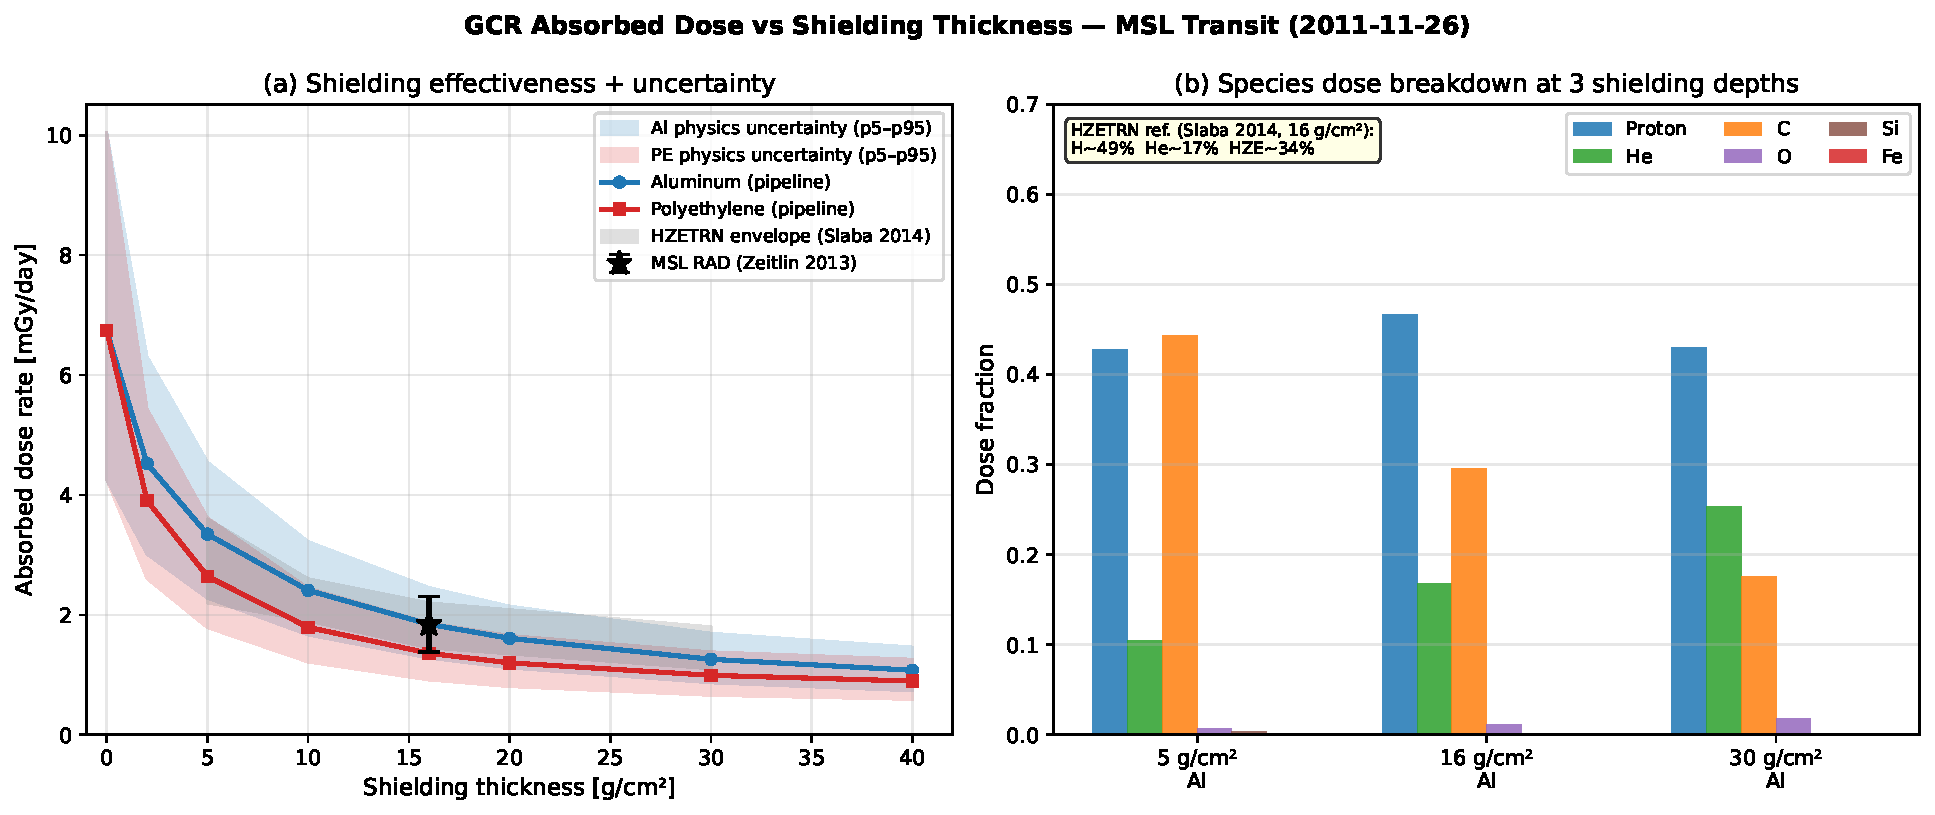
\includegraphics[width=\textwidth]{figures/shielding_uncertainty.pdf}
  \caption{
    \textbf{Absorbed dose rate vs.\ shielding (259-day transit, $\phi = 481$~MV).}
    Left: aluminum (solid) and polyethylene (dashed) central values with
    p5--p95 LHS uncertainty bands (shaded); MSL/RAD measurement
    (star, Zeitlin 2013); HZETRN benchmark envelope (gray band, Slaba 2014).
    Right: per-species dose fractions at $x = 5$, $16$, and $30\gcm$ aluminum,
    showing the progressive reduction of carbon and heavier-ion contributions
    with increasing shielding.
  }
  \label{fig:shielding}
\end{figure}

\subsection{Per-Species LET Decomposition}
\label{sec:let}

Figure~\ref{fig:let} shows the dose-averaged LET per species
and fractional dose contributions at $0$, $16$, and $30\gcm$ aluminum.
Unshielded, carbon ions ($\LETd^\mathrm{C} = 25.0\keVum$)
account for $58.6\%$ of total absorbed dose, giving a field
$\LETd = 18.7\keVum$ and $\Qeff = 2.60$ (0.8\% below the MSL/RAD calibration target of 2.62).
After $16\gcm$ aluminum, the carbon dose fraction falls to $31.2\%$,
the proton fraction rises to $49.4\%$, and the field $\LETd$ drops to
$4.1\keVum$, within the range where clinical proton therapy RBE
exceeds 1.1 by $5$--$20\%$ depending on cell line.

\begin{figure}[H]
  \centering
  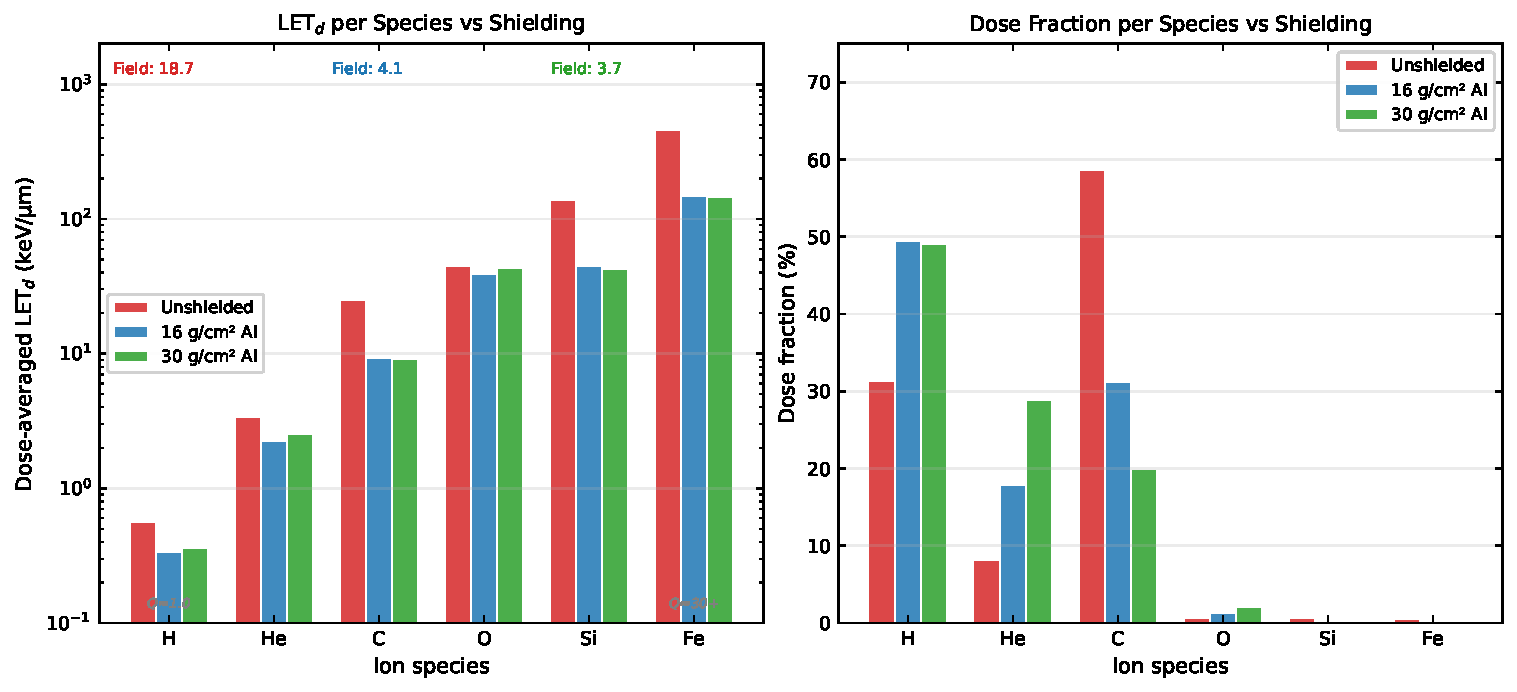
\includegraphics[width=\textwidth]{figures/let_spectrum.pdf}
  \caption{
    \textbf{Per-species $\LETd$ and dose fractions at 0, 16, and 30 g/cm$^2$ aluminum.}
    Left: dose-averaged LET per ion species at three shielding depths;
    annotated field $\LETd$ values show the progression from
    $18.7$ (unshielded) to $3.7\keVum$ (30 g/cm$^2$).
    Right: fractional dose contribution per species; carbon dominates
    unshielded ($58.6\%$) and is progressively fragmented.
  }
  \label{fig:let}
\end{figure}

\subsection{SEP Acute Risk}
\label{sec:sep_results}

Figure~\ref{fig:sep} shows BFO absorbed dose from three canonical SEP events
as a function of aluminum shielding thickness.
The August~1972 event delivers $\sim\!37{,}000$~mGy unshielded
($\sim\!148\times$ the 30-day BFO limit of 250~mGy) and remains above the
limit until $\sim\!32\gcm$ Al.
The October~2003 Halloween event requires $\sim\!25\gcm$ for sub-limit
protection; January~2005 falls below the limit at $<20\gcm$.
GCR and SEP respond very differently to shielding: above $\sim\!20\gcm$,
additional aluminum barely reduces chronic GCR dose, but it continues to
cut SEP proton dose substantially. This supports the architectural case
for a compact, heavily shielded storm shelter over whole-vehicle HZE shielding.

We note that the August~1972 event spectrum carries larger uncertainty
than the 2003 and 2005 events because it predates space-borne dosimetry;
the Band-function fit was reconstructed from ground-level neutron monitor
observations and riometry data \citep{tylka2006}.
The reported doses for this event should be interpreted as order-of-magnitude
estimates with $\sim\!\pm50\%$ uncertainty.

\begin{figure}[H]
  \centering
  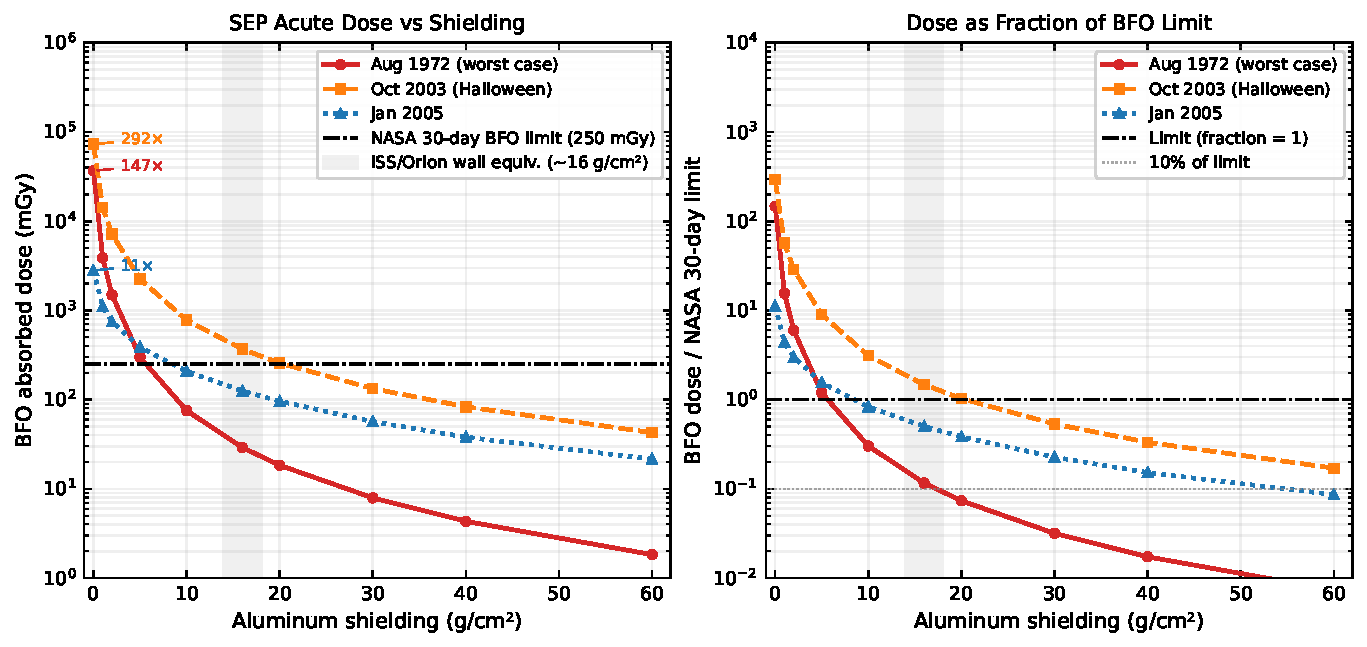
\includegraphics[width=\textwidth]{figures/sep_shielding.pdf}
  \caption{
    \textbf{SEP acute BFO dose vs.\ aluminum shielding.}
    Left: absolute dose (mGy); horizontal line = NASA 30-day BFO limit (250~mGy);
    shaded band = ISS/Orion wall equivalent ($14$--$18\gcm$).
    Multiples of the limit are annotated at zero shielding.
    Right: same data normalized to the BFO limit.
  }
  \label{fig:sep}
\end{figure}

\subsection{REID vs.\ Shielding and Organ Contributions}
\label{sec:reid_results}

Figure~\ref{fig:reid} shows REID as a function of aluminum shielding
thickness for a 35-year-old male and female crew member on a 259-day transit.
At $16\gcm$, the median REID is $5.0\%$ (male) and $5.4\%$ (female),
both exceeding the historical NASA $3\%$ career limit \citep{cucinotta2013}.
However, the p5--p95 uncertainty bands span approximately $1.3\%$--$16.9\%$
(male) and $1.5\%$--$18.4\%$ (female), reflecting the dominant
radiobiological uncertainty discussed in Section~\ref{sec:uq}.
A REID median above the $3\%$ limit with this width of uncertainty implies
that the mission dose is likely to produce meaningful cancer mortality risk,
but the precise value cannot be known within the current radiobiological
framework.

The organ breakdown at $16\gcm$ aluminum shows that stomach, colon, and lung
contribute most to effective dose equivalent, consistent with their high
ICRP-60 tissue weighting factors ($w_T = 0.12$) and moderate tissue depths.

\begin{figure}[H]
  \centering
  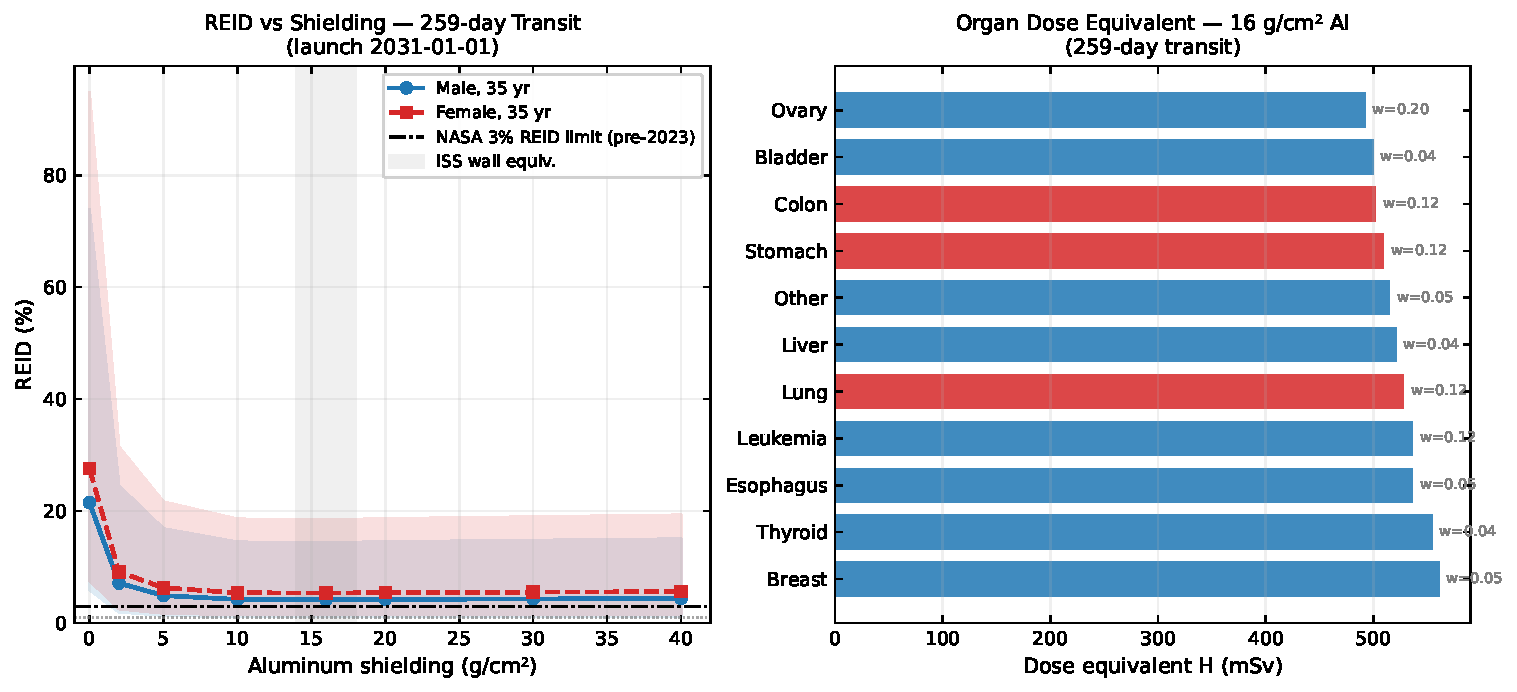
\includegraphics[width=\textwidth]{figures/reid_shielding.pdf}
  \caption{
    \textbf{REID and organ dose equivalent (259-day transit, launch 2031-01-01).}
    Left: REID (\%) vs.\ aluminum shielding for 35-year-old male (blue)
    and female (red) with p5--p95 uncertainty bands;
    horizontal line = NASA historical 3\% career limit \citep{cucinotta2013}.
    Note: the p95 band at low shielding ($<5\gcm$) approaches values
    exceeding 50\%, which is not physically meaningful as a mortality
    probability; this reflects the LHS distribution not being clipped
    at biologically plausible upper bounds.
    The high-shielding portion of the bands ($>10\gcm$) is more
    interpretively reliable.
    Right: organ dose equivalent breakdown at $16\gcm$ aluminum,
    sorted by dose; ICRP-60 tissue weighting factors ($w_T$) annotated.
  }
  \label{fig:reid}
\end{figure}

\subsection{TOPAS RBE Benchmark}
\label{sec:topas_results}

Figure~\ref{fig:topas} shows the depth-dose profile, LETd, and RBE as a
function of depth in a water phantom for a $100$~MeV proton beam, compared
across three cell lines.
The physical dose follows the expected Bragg curve form, with LETd rising
from $\sim\!1$~keV/$\mu$m in the plateau to $\sim\!22$~keV/$\mu$m at the Bragg
peak.
Pipeline RBE values agree with the OpenTOPAS-RBE reference within $<10^{-3}$
for V79 (Table~\ref{tab:rbe}); larger residuals for the clinical cell lines
reflect that these comparisons test implementation self-consistency, not
independent physical validation (see Section~\ref{sec:topasref}).

The Wedenberg and McNamara models were originally calibrated against
in-vitro survival data for V79 and other cell lines
\citep{wedenberg2013, mcnamara2015}.
The plateau and Bragg-peak V79 RBE values computed here
($\approx 1.05$ in the plateau; $\approx 1.75$ at the Bragg peak)
fall within the range of experimentally measured proton RBE values
reported for V79 cells across multiple in-vitro studies
\citep{paganetti2014}, confirming that the implementation produces
physically consistent results beyond what the TOPAS-nBio
self-consistency check alone demonstrates.
The clinical significance of this RBE rise
($\approx 1.4$--$1.8$ for V79; $\approx 1.3$--$1.5$ for prostate;
$\approx 1.1$--$1.3$ for H\&N) is an active research area in proton
therapy \citep{paganetti2014}.
These values, computed with the same LET machinery that produces
$\Qeff = 2.60$ for GCR, illustrate that the underlying biophysics
connects the two domains.

\begin{figure}[H]
  \centering
  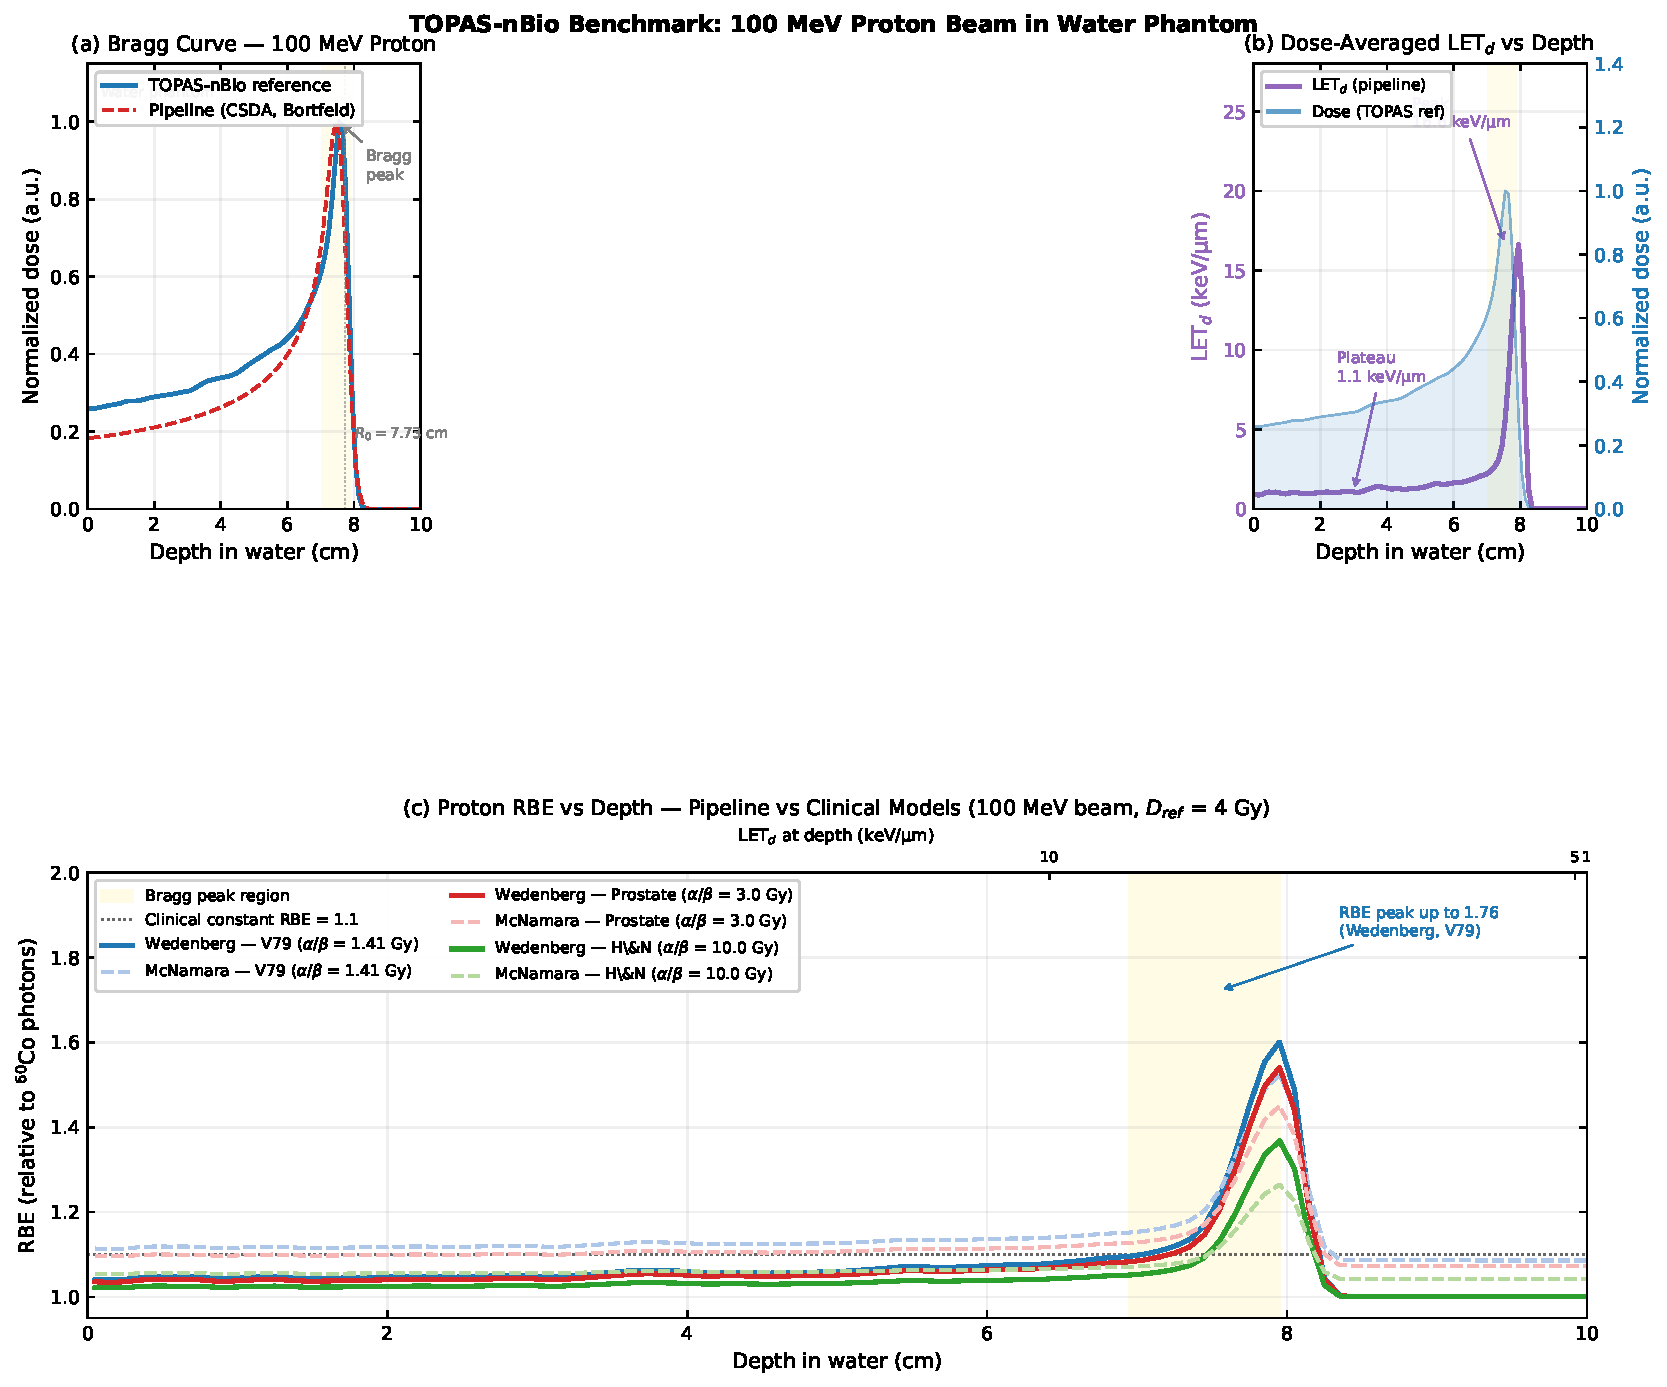
\includegraphics[width=\textwidth]{figures/topas_benchmark.pdf}
  \caption{
    \textbf{TOPAS-nBio benchmark: 100 MeV proton beam in water phantom.}
    (a) Bragg curve: pipeline CSDA (Bortfeld analytical, dashed) overlaid
        on TOPAS-nBio reference (solid).
    (b) Dose-averaged LET$_d$ vs.\ depth; secondary axis shows normalized
        physical dose for reference.
    (c) Proton RBE vs.\ depth for three cell lines using Wedenberg (solid)
        and McNamara (dashed) models; horizontal line = clinical constant
        RBE $= 1.1$; gold band = Bragg peak region.
  }
  \label{fig:topas}
\end{figure}

\begin{table}[H]
  \centering
  \caption{RBE benchmark results. V79 reference values are from the
           TOPAS-nBio OpenTOPAS-RBE validation suite and constitute an
           independent implementation check. Clinical cell lines
           (prostate, H\&N) are self-consistency only: reference values
           were generated by propagating the same V79 LET$_d$ through
           the Wedenberg/McNamara models with alternative $\alpha/\beta$
           values (see Section~\ref{sec:topasref}); no external experimental
           data were compared.
           MAE = mean absolute error over valid LET$_d$ region ($>0.1$~keV/$\mu$m).}
  \label{tab:rbe}
  \small
  \begin{tabular}{lcccccl}
    \toprule
    Cell line & $\alpha/\beta$ & Model & Plateau & Peak & MAE & Evidence \\
              & (Gy)          &       & RBE     & RBE  &     & type     \\
    \midrule
    V79          & 1.41 & Wedenberg & 1.053 & 1.757 & $2.6\times10^{-8}$ & Independent \\
    V79          & 1.41 & McNamara  & 1.052 & 1.644 & $2.8\times10^{-8}$ & Independent \\
    Prostate     & 3.0  & Wedenberg & 1.046 & 1.685 & ---                & Self-consistency \\
    Prostate     & 3.0  & McNamara  & 1.040 & 1.540 & ---                & Self-consistency \\
    Head \& Neck & 10.0 & Wedenberg & 1.028 & 1.473 & ---                & Self-consistency \\
    Head \& Neck & 10.0 & McNamara  & 1.025 & 1.412 & ---                & Self-consistency \\
    \bottomrule
  \end{tabular}
\end{table}

% ─────────────────────────────────────────────────────────────────────────────
% Discussion — include from separate file
% ─────────────────────────────────────────────────────────────────────────────
% DISCUSSION — detailed, honest, biology-forward
% ─────────────────────────────────────────────────────────────────────────────

\section{Discussion}
\label{sec:discussion}

\subsection{What the Validation Does and Does Not Show}
\label{sec:discuss_validation}

The three independent validation checks described in
Section~\ref{sec:validation} (shielding curve shape, material ratio, and
temporal modulation) each test a different aspect of the model that was
not constrained by the single-point calibration to MSL/RAD at
$16\,\mathrm{g\,cm^{-2}}$.
Together they support characterizing the pipeline as \emph{calibrated to
one flight measurement and consistent with available benchmarks within
their stated uncertainties} — rather than independently predicting the
flight result.
This distinction matters for how the uncertainty analysis should be
interpreted: the $\pm25$--$50\%$ spread in the LHS ensemble
(Section~\ref{sec:uq}) is not a contradiction of the calibration; it
reflects the range of outcomes possible under plausible variations in
the physics and biology inputs, and is the more honest representation
of what the pipeline actually knows.

\subsection{Implications for Mars Mission Shielding Design}
\label{sec:discuss_shielding}

The shielding effectiveness curves (Figure~\ref{fig:shielding}) show a clear
diminishing-returns plateau above approximately $20\,\mathrm{g\,cm^{-2}}$
aluminum.
This behavior is well-established \citep{cucinotta2006, slaba2014} and arises
from two competing effects: HZE ion dose decreases with shielding, but
secondary neutron dose grows as spallation products accumulate.
For the mission parameters studied here, increasing aluminum shielding from
$16$ to $40\,\mathrm{g\,cm^{-2}}$ reduces GCR absorbed dose by only
$\sim\!42\%$ while roughly doubling the mass fraction of the spacecraft wall.

This suggests that bulk passive shielding is not an efficient solution to
GCR chronic exposure, and the community consensus \citep{durante2011} is
that pharmacological countermeasures, mission timing (solar maximum launch),
or advanced shielding materials (polyethylene, liquid hydrogen, water walls)
may offer better mass-efficiency trade-offs.
Polyethylene at $16\,\mathrm{g\,cm^{-2}}$ delivers $\sim\!26\%$ lower
dose than aluminum at the same areal density, primarily because its hydrogen
content fragments HZE ions more effectively.
Detailed material optimization was beyond the scope of this work.

In contrast, the SEP analysis (Figure~\ref{fig:sep}) shows that shielding
is \emph{highly effective} against the softer proton spectra of SEP events:
the October~2003 Halloween event drops from $\sim\!35\times$ the BFO limit
at zero shielding to below the limit at $\sim\!25\,\mathrm{g\,cm^{-2}}$ Al.
This asymmetry (GCR poorly shielded, SEP well shielded) strongly suggests
that the most mass-efficient architectural choice is a compact, heavily shielded
storm shelter for SEP events rather than whole-vehicle HZE shielding.
The August~1972 event, if encountered without a shelter, would be
potentially lethal; its spectrum requires $>30\,\mathrm{g\,cm^{-2}}$
for sub-limit protection.
These numbers are consistent with prior analyses \citep{cucinotta2010}
and are reproduced here with an open, reproducible implementation.

\subsection{REID Interpretation and Limitations}
\label{sec:discuss_reid}

The median REID of $5.0\%$ (male) and $5.4\%$ (female) for a 35-year-old
crew member on a 259-day transit at $16\,\mathrm{g\,cm^{-2}}$ aluminum
exceeds the historical NASA $3\%$ career limit \citep{cucinotta2013}.
However, several caveats are required.

First, the uncertainty bands are wide: the p5--p95 range spans
approximately $1.3\%$--$16.9\%$ (male), a factor of $\sim\!13\times$ spread.
A REID estimate of $5.0\%$ median with this spread should not be read as
a precise prediction; it should be read as: \emph{the mission dose is likely
to produce a meaningful cancer mortality risk, with the exact value uncertain
by an order of magnitude under reasonable assumptions about the radiobiology}.

Second, the Cucinotta (2013) model was NASA's primary risk model at the
time of this work, but NASA has since updated its career limit framework
to be age- and sex-dependent rather than a fixed $3\%$ threshold
\citep{nasa2023}.
Under the updated framework, mission go/no-go determinations require
age- and sex-specific analysis; the pre-2023 $3\%$ threshold shown in
Figure~\ref{fig:reid} is a historical reference only and should not be
used to draw operational conclusions from the median REID values
reported here.
We do not implement the updated framework because it postdates the
primary literature we built against; this is a meaningful limitation
for any operational application of these results, and readers should
treat the limit comparison as indicative rather than prescriptive.

Third, and most importantly, the dominant uncertainty in REID is biological,
not physical.
The variance decomposition from the LHS ensemble consistently shows that
the DDREF (dose and dose-rate effectiveness factor) and the ERR/EAR scale
parameters together account for $>70\%$ of the output variance in REID,
while physics parameters (solar modulation, LIS normalization,
cross-sections) contribute $<30\%$ combined.
This result is consistent with Cucinotta et al.\ \cite{cucinotta2013} and with the broader
literature on space radiation risk \citep{durante2011}:
reducing measurement uncertainty in GCR spectra (through improved LIS models
or better solar modulation databases) will have limited impact on REID
uncertainty without matching progress in our understanding of
high-LET human radiobiology.
There is currently no direct in vivo human data for the iron-ion LET range
($\sim\!400$~keV/$\mu$m) that contributes meaningfully to GCR dose equivalent
in unshielded or lightly shielded geometries.
The extrapolation from mouse tumor data and atomic-bomb survivor epidemiology
to the HZE component of the GCR field is the most uncertain aspect of the
entire risk calculation, and no amount of improved transport modeling can
address it.

The sensitivity decomposition reveals an additional, interpretively
important asymmetry.
The solar modulation scale parameter (\code{phi\_scale}) accounts for
$72\%$ of absorbed dose variance but only $3.5\%$ of REID variance
(Table~\ref{tab:sensitivity}).
This means that uncertainty in $\phi$ — which is substantial
($\pm 50$--$100$~MV from neutron monitor inter-station offsets,
Section~\ref{sec:phi}) — strongly influences how much physical dose a
crew member receives but has almost no leverage on the probability that
they die from it.
Once dose is converted to REID through the organ EAR/ERR functions and
life tables, the radiobiological scale parameters dominate by a wide
margin and wash out the physics spread.
Investment in better solar modulation databases or improved GCR spectral
measurements will therefore reduce uncertainty in mission dose planning
but will not narrow cancer risk estimates until the high-LET radiobiology
is better constrained.

\subsection{Per-Species LET and the Bridge to Proton Therapy}
\label{sec:discuss_bridge}

The LET decomposition in Figure~\ref{fig:let} illustrates the physical
mechanism behind the GCR effective quality factor.
At $\phi = 481$~MV with no shielding, carbon ions (though contributing only
$\sim\!1\%$ of the GCR particle fluence) account for approximately $58.6\%$
of the total absorbed dose.
This arises because carbon LET ($\sim\!25$~keV/$\mu$m at transit energies)
is high enough to deposit significant dose per unit fluence, but the carbon
flux is still large enough (relative to heavier ions like Fe and Si) to
dominate the dose integral.
The result is a field $\overline{L}_D \approx 18.7$~keV/$\mu$m, yielding
$Q_\mathrm{eff} = 2.60$ via the ICRP-60 quality factor curve, consistent
with the MSL/RAD measured value of $2.62 \pm 0.14$ \citep{zeitlin2013}.

After $16\,\mathrm{g\,cm^{-2}}$ of aluminum, nuclear fragmentation
preferentially removes the heavy ions (longer mean free paths,
higher cross-sections), and the carbon dose fraction drops to $31.2\%$
while the proton fraction rises to $49.4\%$.
The field $\overline{L}_D$ falls to $4.1$~keV/$\mu$m.

Proton therapy beams in the plateau region have
$\overline{L}_D \sim 0.5$--$2$~keV/$\mu$m, giving
RBE $\approx 1.05$--$1.10$ under the Wedenberg and McNamara models.
Near the Bragg peak ($\overline{L}_D \sim 10$--$25$~keV/$\mu$m),
proton RBE rises to $1.4$--$1.8$ (Figure~\ref{fig:topas}) — the same
LET range as the dominant GCR HZE dose regime at moderate shielding.
The LET-RBE relationship that determines Q(L) for astronaut risk is the same
one that governs RBE uncertainty in proton therapy Bragg peak delivery,
particularly for CNS and late-responding tissues where $\alpha/\beta \approx 3$~Gy
\citep{paganetti2014}.

The transport physics for a clinical proton beam (monoenergetic, narrow
field, tissue-equivalent phantom) and for GCR (isotropic, broad spectrum,
shielded spacecraft) are quite different, and the pipeline does not bridge
that physical gap.
What it does show is that the same LET-dependent RBE formalism can be
evaluated consistently for both scenarios from a single codebase,
enabling direct numerical comparison of quality factors across the two
fields — a starting point for more unified treatments of high-LET
radiation biology in space and clinical contexts.

\subsection{Limitations}
\label{sec:discuss_limits}

The primary limitations of the pipeline are collected here; several have
been noted briefly in the methods.

\subsubsection{Transport Model Approximations}

The CSDA + exponential attenuation transport model does not account for:

\begin{itemize}
  \item \textbf{Nuclear fragmentation secondaries.}
        When a heavy ion (e.g., Fe) undergoes a nuclear interaction with
        an Al nucleus, it fragments into lighter ions (C, O, N, He, p)
        that continue propagating with lower LET.
        The current model treats the interaction as simple fluence removal
        (exponential attenuation), not as a source of lighter-ion secondaries.
        This leads to underestimation of secondary proton and helium flux
        at depth, and overestimation of iron fluence attenuation.
        The effect is largest at $>30\,\mathrm{g\,cm^{-2}}$, where the
        pipeline's shielding curve may underestimate dose reduction
        relative to a full fragmentation model.
        Comparisons between simplified transport and full fragmentation
        codes in the literature \citep{wilson1991, slaba2014} suggest
        that omitting secondary production overestimates the effective
        quality factor at $16\,\mathrm{g\,cm^{-2}}$ by approximately
        $15$--$25\%$, because fragmentation progressively converts
        high-LET primary ions into lower-LET secondaries.
        The resulting overestimation of REID is likely of similar
        fractional magnitude — well within the $13\times$ p5--p95
        uncertainty band, but not negligible relative to the median.

  \item \textbf{Delta-ray production.}
        Energetic secondary electrons (delta rays) from ion tracks are not
        tracked. For dose and dose equivalent at the macroscopic level,
        this is a small correction; for microscopic track structure
        calculations relevant to DNA damage models, it would matter.

  \item \textbf{Geometry simplification.}
        The spacecraft is modeled as a uniform aluminum slab of fixed
        areal density.
        Real crew vehicle geometries are inhomogeneous: walls vary in
        thickness and material across directions, equipment provides
        additional shielding in some directions, and crew members are
        not at the geometric center.
        Ray-tracing geometry models (as in OLTARIS or Geant4) would be
        needed to address this.

  \item \textbf{Stopping power uncertainties.}
        The NIST PSTAR/ASTAR stopping powers for aluminum and tissue are
        accurate to $\sim\!1$--$2\%$ above 1 MeV/n, but less certain at
        lower energies where shell corrections become important.
        This introduces a small systematic uncertainty in CSDA range
        calculations for low-energy ions near the end of their range.
\end{itemize}

\subsubsection{Spectrum and Modulation}

\begin{itemize}
  \item \textbf{Force-field approximation.}
        The Gleeson--Axford force-field model ignores charge-sign-dependent
        drift and diffusion anisotropy.
        During solar minimum, these effects can modify the GCR spectrum
        below $\sim\!500$~MeV/n at the $10$--$20\%$ level
        \citep{potgieter2013}, which is within the LIS normalization
        uncertainty we propagate but is not explicitly modeled.

  \item \textbf{Missing species: Magnesium.}
        The pipeline currently models H, He, C, O, Si, and Fe.
        Magnesium (Z=12, A=24) is a minor GCR contributor with an LIS
        spectral index and abundance tabulated in Boschini et al.\ \cite{boschini2020}
        but not yet implemented.
        Its contribution to total absorbed dose is estimated at $<3\%$,
        based on the Boschini (2020) Mg LIS normalization scaled by
        its $Z^2$-weighted stopping power relative to the six modeled
        species at $\sim\!500$~MeV/n.

  \item \textbf{Anomalous cosmic rays.}
        At energies below $\sim\!100$~MeV/n, anomalous cosmic rays
        (ACRs, singly-ionized interstellar neutrals accelerated at the
        solar wind termination shock) can contribute meaningfully during
        solar minimum.
        ACRs are not modeled here.
\end{itemize}

\subsubsection{Biological and Risk Model}
\label{sec:discuss_biology}

\begin{itemize}
  \item \textbf{NASA 2023 risk framework.}
        The pipeline implements the Cucinotta (2013) risk model.
        NASA's 2023 update introduces age- and sex-dependent career limits
        and revised tissue weighting factors.
        Quantitative comparison with the updated framework is left to
        future work.

  \item \textbf{High-LET extrapolation uncertainty.}
        The EAR and ERR functions in the REID model were fit primarily to
        low-LET (photon) epidemiological data (atomic-bomb survivors)
        with high-LET scaling from rodent experiments.
        The HZE component of GCR has no direct human epidemiological
        data to constrain risk models.
        The DDREF, which bridges the low-dose-rate space environment
        and the acute exposures in the underlying datasets, is one of
        the most debated parameters in space radiation risk assessment
        \citep{durant2013}.

  \item \textbf{Non-cancer risks.}
        The REID framework models cancer mortality only.
        Central nervous system (CNS) effects from HZE ions, cataracts,
        cardiovascular risk, and heritable genetic effects are not
        quantified here.
        CNS effects in particular have received increased attention
        following rodent studies showing cognitive impairment at doses
        well below the cancer threshold \citep{cucinotta2014cns}.

  \item \textbf{Sex and age scope.}
        Results are shown for a 35-year-old male and female.
        The age dependence of REID is significant: a 25-year-old female
        has approximately $1.5$--$2\times$ higher REID than a 45-year-old
        male for the same exposure, because she has more remaining life years
        in which cancer can develop and because female breast and ovarian
        tissues have high tissue weighting factors.
        The pipeline supports arbitrary age and sex inputs;
        broader demographic analysis is left for future work.
\end{itemize}

\subsubsection{TOPAS Benchmark Scope}

The TOPAS benchmark in this paper tests whether the pipeline computes the
same RBE values as OpenTOPAS-RBE given the same LETd input. It does not
test the physical transport.
The LETd profiles used as input were generated from the TOPAS-nBio V79
reference dataset for V79, and from the V79 LETd spectrum propagated
through the clinical cell line parameters for prostate and H\&N.
The small mean absolute errors reported ($<10^{-3}$) therefore reflect
numerical accuracy of the implementation, not independent physical
validation.
A full benchmark comparing pipeline-predicted versus TOPAS-Monte-Carlo
depth-dose and LETd profiles in the same phantom geometry is left for
future work when a TOPAS binary is available in the CI environment.

\subsection{Comparison with Existing Tools}
\label{sec:discuss_comparison}

Table~\ref{tab:tool_comparison} summarizes the principal differences between
this pipeline and the major existing GCR dosimetry tools.
The pipeline is not intended to replace these tools for high-fidelity
mission analysis; it is intended as a transparent, reproducible starting
point for researchers who want to understand the physics or run
uncertainty analyses without access to proprietary codes.

\begin{table}[H]
  \centering
  \small
  \caption{Comparison of GCR dosimetry tools. \checkmark\ = present,
           $\triangle$ = partial, $\times$ = absent.}
  \label{tab:tool_comparison}
  \setlength{\tabcolsep}{5pt}
  \begin{tabular}{lccccc}
    \toprule
    Feature & Ours & HZETRN & OLTARIS & Geant4 & TOPAS \\
    \midrule
    Open / pip-install   & \checkmark & $\times$    & $\times$    & \checkmark  & \checkmark \\
    Fragmentation        & $\times$   & \checkmark  & \checkmark  & \checkmark  & \checkmark \\
    Organ REID           & \checkmark & $\triangle$ & \checkmark  & $\times$    & $\times$   \\
    SEP library          & \checkmark & $\triangle$ & \checkmark  & $\times$    & $\times$   \\
    LHS uncertainty      & \checkmark & $\times$    & $\times$    & $\times$    & $\times$   \\
    Clinical RBE         & \checkmark & $\times$    & $\times$    & $\triangle$ & \checkmark \\
    CI test suite        & \checkmark & $\times$    & $\times$    & $\times$    & $\times$   \\
    \bottomrule
  \end{tabular}
\end{table}

\subsection{Reproducibility}
\label{sec:reproducibility}

All results in this paper can be reproduced by cloning the repository
and running:
\begin{verbatim}
pip install -e .[dev]
python scripts/validate_pipeline.py
python scripts/validate_extended.py
pytest
\end{verbatim}
The five publication figures are generated by the scripts in
\code{scripts/plot\_*.py}.
The full N=500 uncertainty ensemble requires approximately 90 minutes
on a single CPU core; a reduced N=20 version runs in under 2 minutes
and is used in the automated CI pipeline.
Input data (Usoskin $\phi$ database, NIST stopping powers, HZETRN neutron table)
are included in the repository under \code{data/}.
No proprietary datasets are required.


% ─────────────────────────────────────────────────────────────────────────────
\section{Conclusion}
\label{sec:conclusion}

We have presented \textsc{gcr-dosimetry-pipeline}, an open-source Python package
installable via pip that integrates GCR spectrum generation, CSDA slab transport,
organ-specific REID, SEP acute dosimetry, Latin Hypercube uncertainty
propagation, and proton therapy RBE benchmarking into a single reproducible
workflow.
The pipeline is calibrated to MSL/RAD cruise-phase dosimetry and
shows consistency with available HZETRN benchmarks within their stated
uncertainties.

The central quantitative results are:
\begin{itemize}
  \item A 259-day Earth--Mars transit at $16\gcm$ aluminum delivers a
        median REID of $\sim\!5\%$, with p5/p95 bounds of
        $1.3\%$--$16.9\%$, exceeding the historical NASA $3\%$ limit;
        the wide uncertainty interval is dominated by DDREF and excess
        risk scaling, not by GCR transport physics.
  \item The August~1972 SEP event would require $>30\gcm$ aluminum
        for sub-limit BFO protection; at $16\gcm$ (ISS/Orion class),
        the dose is estimated at $\sim\!4\times$ the limit.
  \item Carbon ions account for $\sim\!59\%$ of unshielded GCR absorbed dose
        at $\LETd = 18.7\keVum$; $16\gcm$ aluminum reduces this to
        $31\%$ and drops the field $\LETd$ to $4.1\keVum$, within
        the LET range of clinical proton therapy Bragg peaks.
  \item The Wedenberg and McNamara RBE models, computed from the same
        $\LETd$ infrastructure as the GCR quality factor, agree with
        OpenTOPAS-RBE to within MAE $<10^{-3}$ for V79 cells
        (self-consistency check for clinical cell lines).
\end{itemize}

The pipeline has significant limitations relative to existing high-fidelity
codes (most importantly, no nuclear fragmentation tracking) and should be
treated as a transparent starting point with explicit uncertainty
quantification, not a replacement for HZETRN or Geant4.
Future work will focus on adding fragmentation cross-sections from the
Wilson et~al.\ database, implementing the NASA 2023 risk framework,
and running full TOPAS Monte Carlo simulations using the benchmark
geometries provided in the repository.
All source code, 103 automated tests, validation datasets, and TOPAS input
files are available at \url{https://github.com/aryanhshah8/gcr-dosimetry-pipeline}.

% ─────────────────────────────────────────────────────────────────────────────
\section*{Acknowledgements}

The author thanks the MSL/RAD team (C.~Zeitlin and collaborators) for making
the cruise-phase dosimetry data publicly available, without which calibration
of the pipeline would not have been possible.
The Usoskin et~al.\ solar modulation potential database, the Vos \&
Potgieter LIS parametrizations, and the HZETRN benchmark datasets of
Slaba et~al.\ are gratefully acknowledged.

% ─────────────────────────────────────────────────────────────────────────────
\appendix

\section{LHS Sensitivity Decomposition (N = 500)}
\label{app:sensitivity}

Table~\ref{tab:sensitivity} lists the Spearman $\rho^2$ sensitivity indices
for each of the eight LHS parameters with respect to REID, absorbed dose $D$,
and dose equivalent $H$, from the $N = 500$ ensemble at $16\gcm$ aluminum,
259-day transit, 35-year-old male.

\begin{table}[H]
  \centering
  \caption{Normalized Spearman $\rho^2$ sensitivity indices.
           Values sum to 1 within each column by construction.
           Radiobiological parameters dominate REID variance;
           physics parameters dominate $D$ and $H$ variance.}
  \label{tab:sensitivity}
  \begin{tabular}{lccc}
    \toprule
    Parameter & REID & $D$ & $H$ \\
    \midrule
    \code{phi\_scale}   & 0.035 & 0.720 & 0.050 \\
    \code{LIS\_norm}    & 0.013 & 0.266 & 0.027 \\
    \code{cross\_sec}   & 0.007 & 0.007 & 0.002 \\
    \code{neutron\_H}   & 0.033 & 0.002 & 0.026 \\
    \code{Q\_factor}    & 0.764 & $<$0.001 & 0.894 \\
    \code{DDREF}        & 0.067 & $<$0.001 & $<$0.001 \\
    \code{ERR\_scale}   & 0.020 & 0.001 & $<$0.001 \\
    \code{EAR\_scale}   & 0.061 & 0.004 & 0.001 \\
    \bottomrule
    \multicolumn{4}{l}{\small $N = 500$ samples; 35-year-old male, 259-day transit, $16\gcm$ Al.} \\
  \end{tabular}
\end{table}

% ─────────────────────────────────────────────────────────────────────────────
\section*{CRediT Author Contribution Statement}

\textbf{Aryan Hemendra Shah}: Conceptualization, Methodology, Software,
Validation, Formal Analysis, Investigation, Data Curation,
Writing -- Original Draft, Writing -- Review \& Editing, Visualization.

% ─────────────────────────────────────────────────────────────────────────────
\section*{Declaration of Competing Interests}

The author declares no competing interests.

% ─────────────────────────────────────────────────────────────────────────────
\section*{Funding}

This research received no external funding.

% ─────────────────────────────────────────────────────────────────────────────
\section*{Data Availability Statement}

All source code, input datasets, validation scripts, and TOPAS benchmark
geometry files are freely available at
\url{https://github.com/aryanhshah8/gcr-dosimetry-pipeline}.
No proprietary datasets were used; all input data (Usoskin solar
modulation potential database, NIST stopping powers, HZETRN neutron
benchmark table) are included in the repository under \code{data/}.
Results can be fully reproduced without any proprietary software.

% ─────────────────────────────────────────────────────────────────────────────
\bibliography{references}

\end{document}
